\lstset
{
    basicstyle=\footnotesize,
    numbers=left,
    stepnumber=1,
    showstringspaces=false,
    tabsize=1,
    breaklines=true,
    breakatwhitespace=false,
}


\begin{figure}[H]
    \centering
    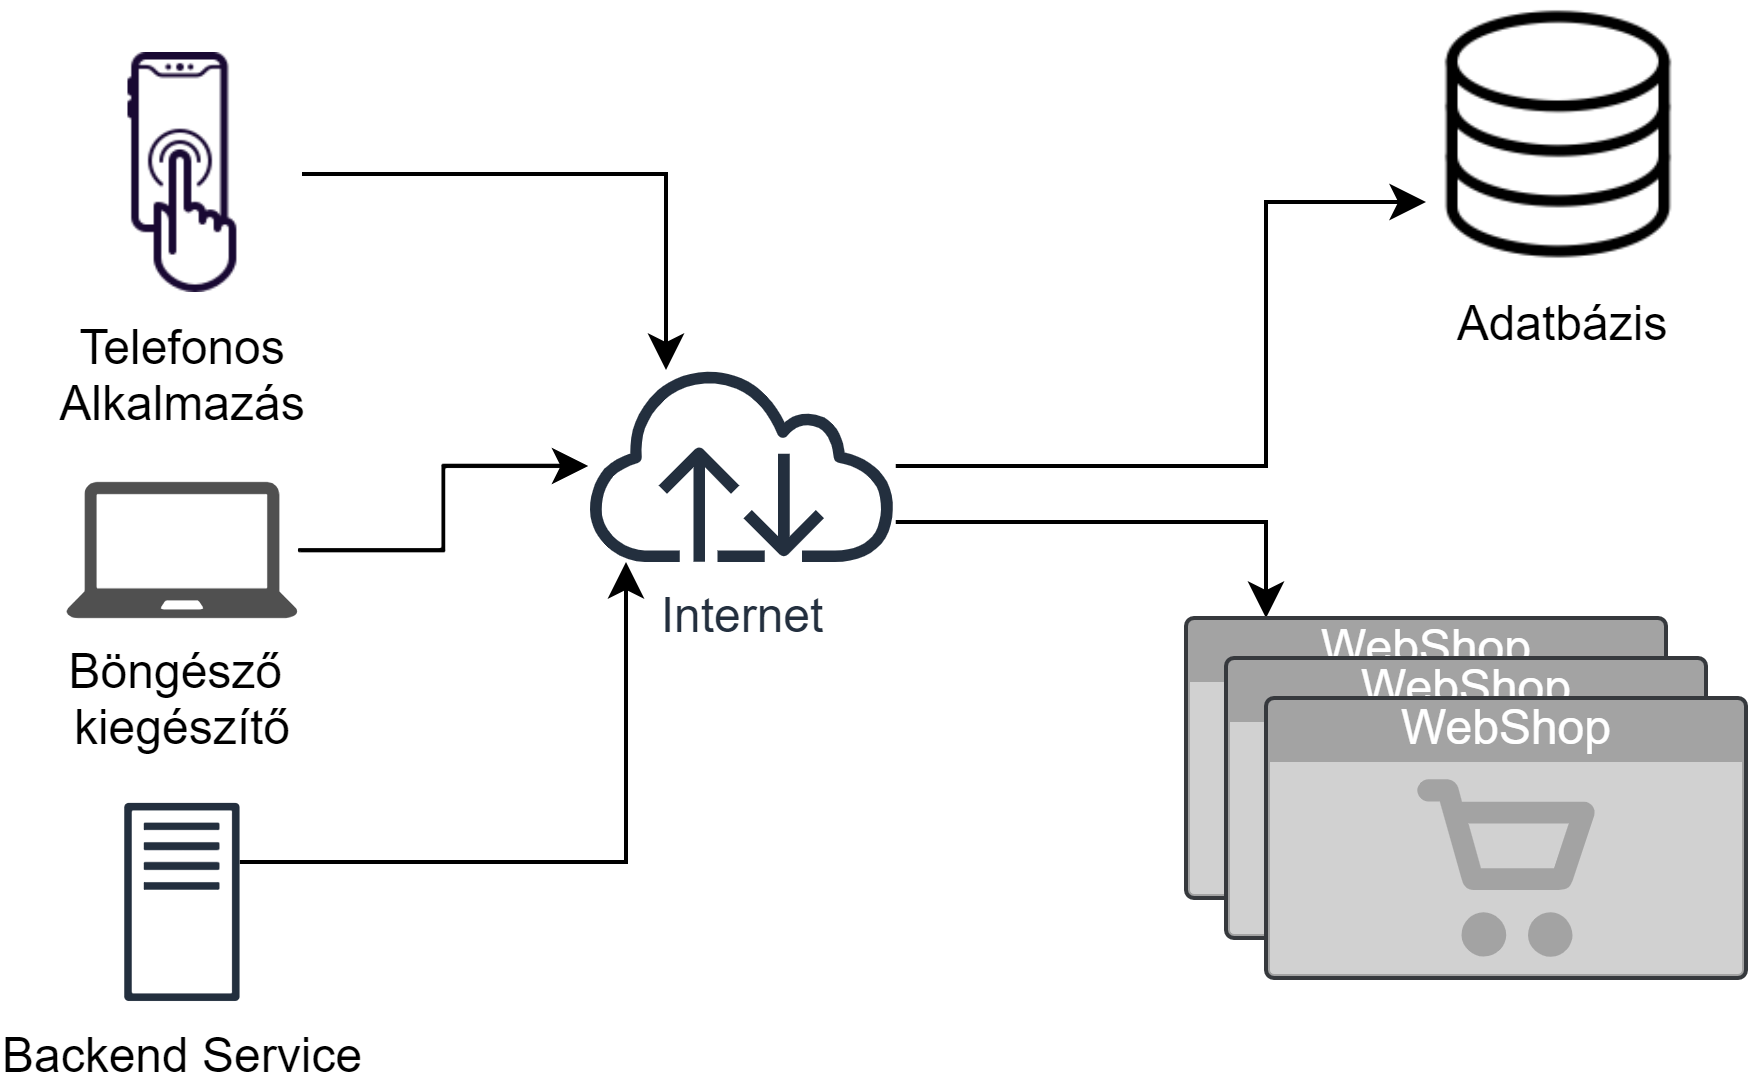
\includegraphics[scale=1.2]{figures/images/architecture_horizontal_HU.png}
    \caption{A rendszer architektúrája}
    \label{fig:architecture}
\end{figure}

A rendszer alapvető részét képezi az adatbázis, amely az adatok tárolását, illetve az azokat elérő API-t szolgáltatja. Ehhez az adatbázishoz két alapvető típusú készülék csatlakozik. A felhasználó oldali, amely lehet akár böngésző kiegészítő vagy telefonos alkalmazás, illetve a szerver vagy logika oldali, amely az adatok feldolgozását biztosító logikát és erőforrást tartalmazza, utóbbi a \ref{fig:architecture} ábrán Backend Service-ként van jelölve. 

A böngésző kiegészítő szükséges, mivel sokkal gyorsabban el lehet érni a megtekinteni kívánt adatokat, valamint sokkal egyszerűbbé teszi a termékek hozzáadását azzal, hogy a követni kívánt termék oldalát egyáltalán nem kell elhagyni. Továbbá fontos, hogy az alkalmazás tudja azt, hogy a felhasználó épp milyen oldalon tartózkodik, ahhoz, hogy a megfelelő URL-t kapja meg, mindezt a kiegészítő könnyen és megbízhatóan el tudja végezni.

Mivel azonban nem mindig vagyunk laptop vagy asztali gép közelben, ezért lehetőséget nyújtunk arra, hogy telefonos applikáció segítségével is el lehessen érni a követett termékeket, valamint minden ehhez tartozó műveletet, akárcsak az előbb említett kiegészítő esetén. Egy termék hozzáadása ezúttal az operációs rendszer megosztási menüjén keresztül történik, ami által az alkalmazás megkapja a követni kívánt termék elérhetőségét.

Ahhoz, hogy az eszközök kommunikálni tudjanak egymással, egyértelmű, hogy szükség van valamiféle összeköttetésre, amely a mi esetünkben az Internet lesz. Ez a funkció létfontosságú, mivel minden adatot fel, illetve le kell tölteni az adatbázisból, függetlenül az eszközök tartózkodási helyétől, ugyanakkor a szolgáltatást biztosító rendszer is ezen keresztül éri el a termékek weboldalát.

Az architektúra fontos részét képezik a webshop-ok is, mivel ezeket úgy a termék hozzáadásakor, mint azoknak periodikus ellenőrzésekor el kell érni, az adatok begyűjtése érdekében. A támogatott webshop-ok főként népszerűségüket tekintve lettek kiválasztva. Mivel minden weboldal másképp épül fel, mindegyik oldal struktúrájából másképp kell kinyerni az adatokat, ezért ezt a folyamatot személyre szabottan kell végezni. Ugyanakkor változhatnak is idővel ezek a struktúrák, ezeket folyamatosan figyelni kell. 

\section{A modulok megvalósítása}

\subsection{Chrome Extension}

A böngésző kiegészítő vagy angolul browser extension, egy a böngésző környezetén belül futó alkalmazás, ami olyan funkciókat hivatott hozzáadni a felhasználói felülethez, melyek megkönnyítik vagy jobbá teszik a felhasználói élményt. Előnye, hogy alkalmazások ezrei állnak a felhasználok rendelkezésére, melyeket pár kattintással telepíthetnek is. Ezek már szinte minden böngészőn megtalálhatók valamilyen formában, a legnépszerűbbek esetében, mint például, Google Chrome, Firefox ez a funkció régóta jelen van.

Ezen kiegészítők működése valószínűleg sokak számára ismert, amolyan lenyíló ablakként jelennek meg a böngészőben, anélkül, hogy hatással lennének az éppen megjelenített tartalomra. Ennek tudatában, ez a megközelítés tűnt a legmegfelelőbbnek a dolgozatban tárgyalt szoftver felhasználói felületének elkészítése során. Mivel ezek a funkciók csak asztali gépeken érhetőek el, ezért szükséges volt egy telefonos interface kifejlesztése is, mely a későbbiekben kerül bemutatásra.

A kiegészítő megvalósítása során, JavaScript, HTML, CSS programozási nyelvek voltak felhasználva. Mivel korábban nem volt tapasztalatom böngészőhöz való kiegészítők fejlesztésében, ezért az implementálási folyamat információ gyűjtéssel kezdődött.

Első lépésben szükséges egy manifest.json file létrehozása, mely a kiegészítő alapvető információit tartalmazza, mint például verziószám, név, rövid leírás, felhasznált függőségek, engedélyezett műveletek stb... . Ezek után, a fejlesztés hasonló egy hagyományos weboldal elkészítéséhez. 

% \begin{lstlisting}[caption={manifest.json file}, label={lst:manifest}, basicstyle=\footnotesize]
%     {
%         "manifest_version": 2,
%         "name": "Price Monitor",
%         "description": "Price monitoring interface",
%         "version": "0.9",
%         "icons": {"128": "icons/icon128.png"},
%         "browser_action" : {
%             "default_icon": "icons/icon19.png",
%             "default_popup": "login.html"
%         },
%         "content_scripts":[{
%             "matches":["<all_urls>"],
%             "js": ["content.js"]
%         }],
%         "background": {
%             "page": "background.html"
%         },
%         "permissions": ["storage", "unlimitedStorage", "tabs", "activeTab", "<all_urls>"],
%         "content_security_policy": "script-src 'self' https://cdn.amcharts.com/lib/4/core.js https://cdn.amcharts.com/lib/4/charts.js https://cdn.amcharts.com/lib/4/themes/dataviz.js https://cdn.amcharts.com/lib/4/themes/animated.js https://www.gstatic.com/ https://*.firebaseio.com https://apis.google.com https://www.googleapis.com https://securetoken.googleapis.com; object-src 'self'; connect-src 'self' https://securetoken.googleapis.com https://apis.google.com https://www.googleapis.com wss://*.firebaseio.com"
%     }
% \end{lstlisting}

\lstinputlisting[caption={manifest.json file}, label={lst:manifest}]{E:/1.UniFuckinVersity/Allamvizsga/Extensions/Chrome/manifest.json}

A fejlesztés során több könyvtár került felhasználásra, különböző funkciók ellátására, ezek a Bootstrap\footnote{\url{https://getbootstrap.com/}}, sweetalert2\footnote{\url{https://sweetalert2.github.io/}}, firebase\footnote{\url{https://firebase.google.com/}}, amcharts\footnote{\url{https://www.amcharts.com/}}. A bootstrap egy ingyenes, nyílt forráskádul CSS framework, mely segítségével interaktívabbá, szebbé tehetjük a weboldalunkat, előre definiált mintákat biztosit nekünk, gombok, navigáció vagy más komponensek esetében. A sweetalert2 egy úgynevezett riasztásokért felelős könyvtár, olyan esetekben került használatra, amikor egy felugró ablak segítségével szeretnénk megerősítést kérni a felhasználótól egy bizonyos művelet elvégzésére, mint például termékek törlése vagy kijelentkezés során, viszont egyéb, információ közlési célokra is felhasználva lett, mint például egy művelet sikeres elvégzésének visszajelzése. A firebase könyvtárakat bejelentkezési, valamint adatbázis kezelő funkciók miatt volt szükséges használni. Az árak időbeli változását ábrázoló diagramok eseteben több könyvtárat is kipróbáltam (Chart, Highcharts, ApexCharts), viszont a végső választás az amCharts nevűre esett, mivel ez volt a leg megfelelőbb az adott esetben, főleg az úgynevezett „panning” funkció miatt, mely lehetővé teszi hogy görgessünk a diagramon, illetve az idő skálát is változtatni tudjuk, mindezt valós időben. Ezen funkciók segítségével pontosabban és hatékonyabban tudjuk követni az árak változását, ugyanakkor vizuális szempontból is kellemes élményt nyújt.

Amikor a felhasználó először használja a kiegészítőt, egy login oldal jelenik meg számára, melyen be tud jelentkezni, valamint regisztrálni tud (\ref{fig:ext_login_reg} ábra).

\begin{figure}[H]
    \centering
    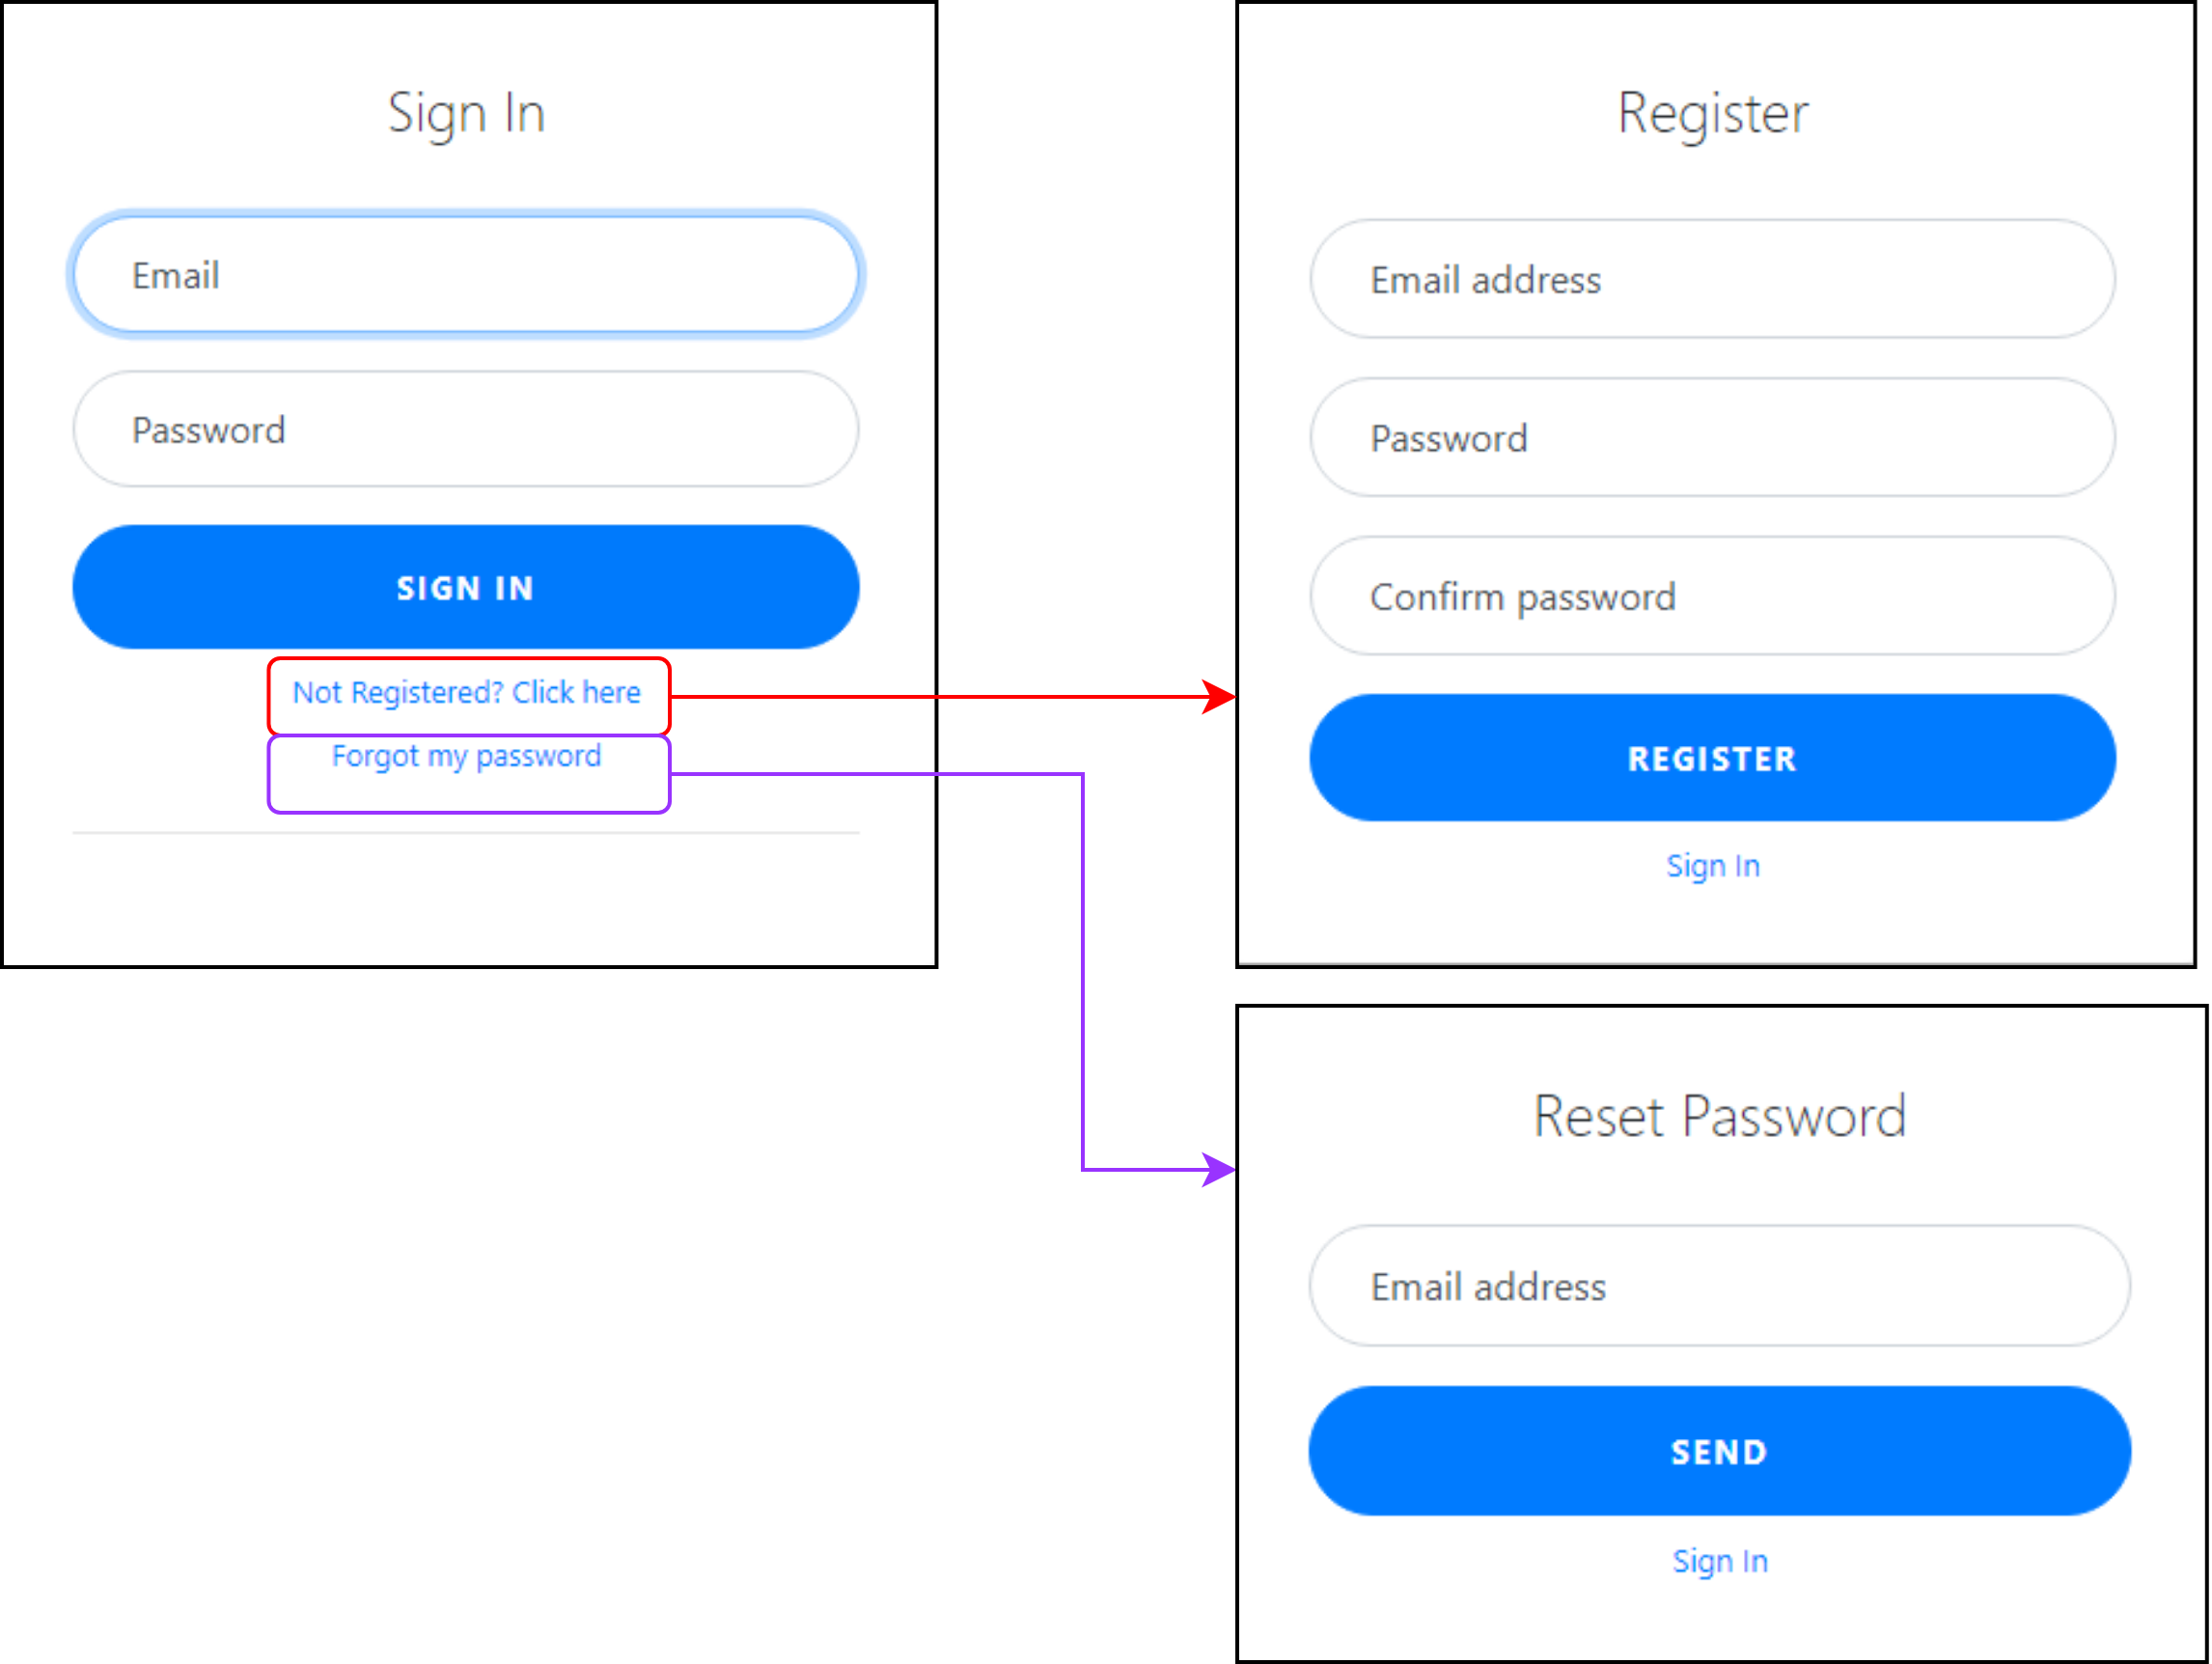
\includegraphics[scale=1]{figures/images/login-reg-ext.png}
    \caption{Kiegészítő bejelentkezési/regisztrálási felülete}
    \label{fig:ext_login_reg}
\end{figure}

Bejelentkezés után a felhasználó a főoldalon találja magát, ahol megtekintheti a követett termékeit, ugyanakkor az alkalmazás használatával kapcsolatos információkat is megtalálja, a fejlécben található “i” szimbólummal jelölt gombra kattintva, valamint ugyanitt vannak felsorolva a támogatott oldalak, melyekre kattintva, az adott weboldalra navigálhatunk. A jelenleg támogatott webshopok az Emag\footnote{\url{https://www.emag.ro/}}, Flanco\footnote{\url{https://www.flanco.ro/}} és QuickMobile\footnote{\url{https://www.quickmobile.ro/}}. Továbbá, szintén a fejlécben található a felhasználó fiókjához tartozó információkat elérő gomb, melynek hatására egy felrúgó ablakban tekintheti meg az email címet, amivel bejelentkezett, illetve itt tud adminisztrációs műveleteket is végezni. Az előbb tárgyaltokat \ref{fig:ext_homescreen_info_user} ábrán láthatjuk.

Új termék hozzáadásakor, az ablak tetején található „Track product on this page” gombra kattintva (\ref{fig:ext_homescreen_info_user} ábra) tehetjük ezt meg, melyek után pillanatokon belül látható majd a listában az adott termék. Amennyiben nem az alkalmazás által nem támogatott oldalon tartózkodunk, ez az opció nem elérhető, a gomb egyszerűen nem jelenik meg. Amikor követni szeretnénk egy termeket, az alkalmazás beszúrja a termék URL-jét az adatbázisba, ami után majd az szoftver backend része végzi majd az információk lekérését, erről később részletesen is szó lesz.

\begin{figure}[H]
    \centering
    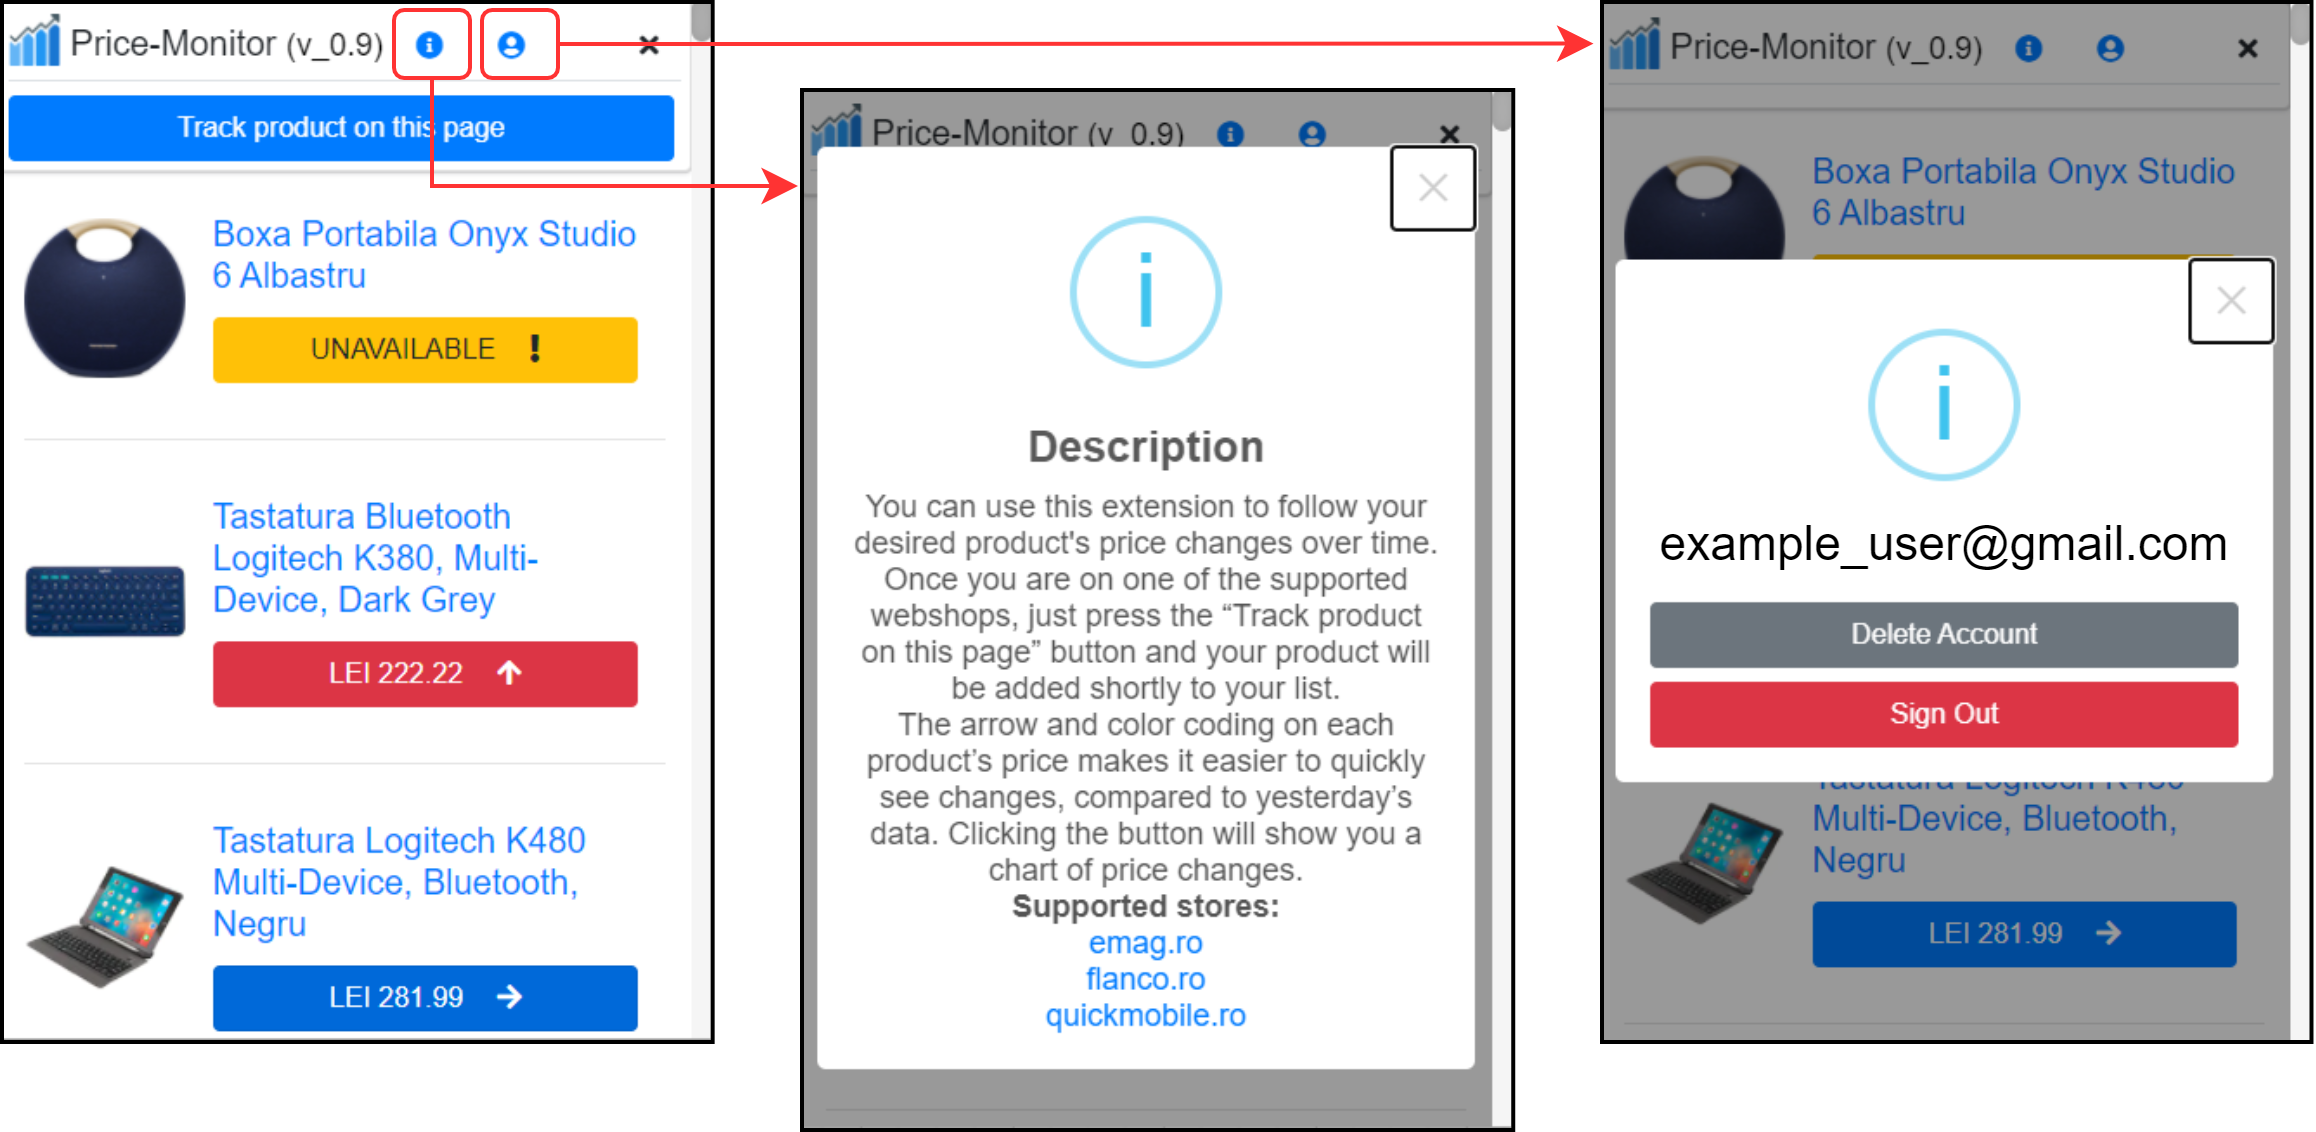
\includegraphics[scale=1.15]{figures/images/home_info_user.png}
    \caption{Főoldal, adminisztrációs rész}
    \label{fig:ext_homescreen_info_user}
\end{figure}

Amint a \ref{fig:ext_homescreen_info_user} ábrán is láthatjuk, a termékek gombjai tartalmazzák a termék aktuális árát, tőlük jobbra egy nyilat, valamint ezek különböző színűek. A nyilak, illetve, színkódolás azért van, hogy a felhasználónak visszajelzést adjuk arról, hogy a termék drágult, olcsóbb lett, nem változott az ára, esetleg jelenleg nem elkérető. Amennyiben a termék drágul, ezt egy felfele mutató nyíl és piros szín jelzi, csökkenés esetén a nyíl lefele mutat és a gomb színe zöldre vált, az utóbbi az \ref{fig:ext_chart} ábrán látható. Amikor egy termék ára nem változik, ezt egy vízszintesen irányuló nyíl és a kék szín jelzi, valamint, ha a termék nem elérhető, akkor ezt sárga szín és az „UNAVAILABLE” szöveg mutatja.

Ha egy termék gombjára kattintunk, akkor megnézhetjük az adott termék arának változását egy diagramon, a követés pillanatától az aktuális dátumig. Amint a \ref{fig:ext_chart} ábra mutatja, a diagramon szépen látható az arák változása, ami sok esetben naponta akár többször is változhat. Mivel az adatmennyiség idővel nagyon nagy lehet, ezért a diagramot mozgatni lehet, hogy egy adott intervallumot vizsgáljunk, vagy az időskálát növelhetjük, illetve csökkenthetjük, igénynek megfelelően, a diagram tetején található csúszka segítségével. Láthatjuk továbbá azt is, hogy ha az egeret a diagram egy adott pontján tartjuk, akkor az levetíti nekünk az adott dátumon a termék árát. Az ablak alján található a törlés gomb, ezzel törölhetjük a terméket a listánkból, ha esetleg már nem vagyunk érdekeltek az adott árucikk követesében. Az előbb említett törlés gomb fölött helyezkedik el még egy gomb, mely megnyomásával az adott termék weboldala nyílik meg számunkra a böngésző egy új ablakában.

\begin{figure}[H]
    \centering
    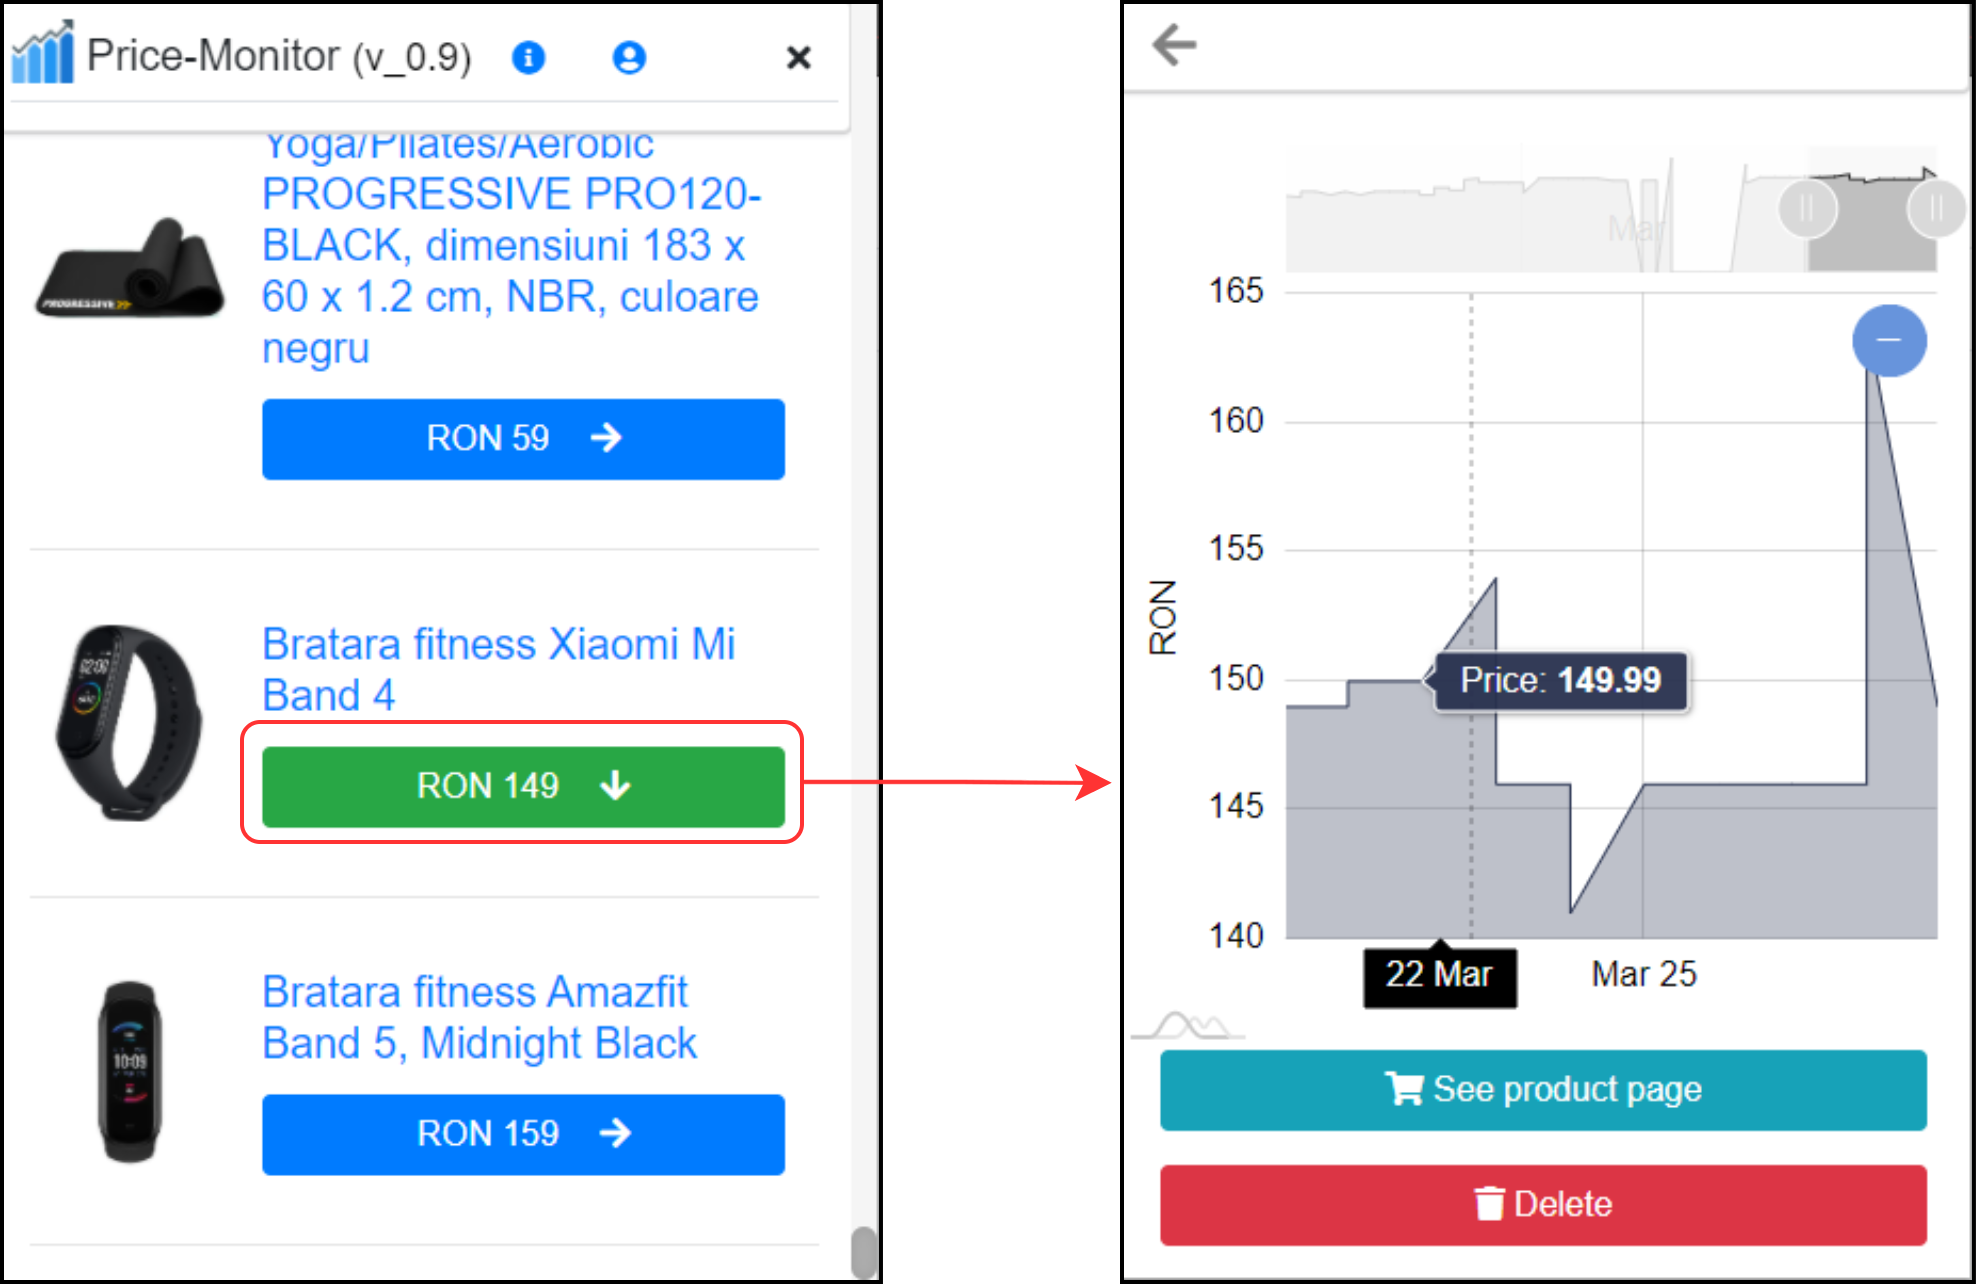
\includegraphics[scale=1]{figures/images/home_details.png}
    \caption{Termék árváltozása}
    \label{fig:ext_chart}
\end{figure}

A diagram megvalósítása az amcharts nevű könyvtárral történt, mely a mi felhasználásunkra tökéletesnek minősült, minden funkciót hozva, amely megkönnyíti az adatok megtekintését, elemzését. Első lépésben az adathalmaz került létrehozásra és formázásra, annak megfelelően, ahogy az adott diagram elvárja azt (Listing \ref{lst:create_chart_data}).

\lstinputlisting[caption={Adathalmaz létrehozása}, label={lst:create_chart_data}, firstline=15, lastline=18]{E:/1.UniFuckinVersity/Allamvizsga/Extensions/Chrome/chart.js}

Következő lépésben maga a diagram lett létrehozva a különböző beállításokkal együtt, mint például időskála formázása, tengelyek elnevezése, a diagram kezdeti állapota, ezt a \ref{lst:create_chart} kódrészlet valósítja meg.

\lstinputlisting[caption={Diagram létrehozása, beállitása}, label={lst:create_chart}, firstline=20, lastline=51]{E:/1.UniFuckinVersity/Allamvizsga/Extensions/Chrome/chart.js}

\subsection{Telefonos alkalmazás}

A telefonos alkalmazás Flutterben került megvalósításra. A Flutter\footnote{\url{https://flutter.dev/}} egy nyílt forráskódú szoftver fejlesztési csomag, melyet a Google hozott a piacra 2018-ban és főként felhasználói felületek fejlesztésére alkalmazzák. Az utóbbi időben rendkívül nagy népszerűségnek örvend a platform, mivel széleskörű felhasználása van. Segítségével Android, iOS, Windows, Mac, Linux valamint a kevésbé ismert Google Fuchsia alatt futó alkalmazásokat lehet fejleszteni, amelyeket egyetlen kódbázisból állít elő, azaz nem szükséges minden egyes platformra külön-külön megírni ezeket.

A Flutter alkalmazások Dart nyelven íródnak, mely szintén a Google által fejlesztett objektum orientált, osztály alapú programozási nyelv, ami 2013 debütált, viszont csak évekkel később terjedt el szélesebb körben.

A Flutter sajátossága az úgynevezett “Hot Reaload”, mely lehetővé teszi a futás közbeni változtatások elvégzését, ami nagyban felgyorsítja a fejlesztési folyamatot, hiszen nem kerül az egész alkalmazás újra kompilálásra. Ezt a “just-in-time” kompilálás teszi lehetővé, melyet más nevén dinamikus fordításnak is neveznek, lényege hogy a kód futás közben kerül kompilálásra és nem pedig az alkalmazás indítása előtt. A platform egy Widget alapú megközelítést alkalmaz, azaz több definiált komponenst biztosít ahhoz, hogy felépítsük az általunk megvalósítani kívánt alkalmazást.

A telefonos alkalmazás fejlesztése Android Studio integrált fejlesztői környezetben történt, felhasználva az általa biztosított Android Emulator programot is, mely segítségével egy telefont lehet emulálni, annak érdekében, hogy az alkalmazást minél valósabb környezetben lehessen fejleszteni, minél változatosabb specifikációjú telefonon lehessen kipróbálni, természetesen ez fizikai telefonon is végezhető. A fejlesztés során úgy virtuális, mint fizikai környezetben is periodikusan ellenőrizve lett az alkalmazás.

Első lépéseben az alkalmazás bejelentkezési funkciója lett megvalósítva, amely a flutter\textunderscore login\footnote{\url{ https://pub.dev/packages/flutter_login}} nevű könyvtár segítségével történt, mivel ez nagyban felgyorsította a fejlesztést, ugyanakkor komplexebb funkcionalitásokat illetve vizuális hatásokat is tartalmaz, melyek kellemesebbé teszik a felhasználói élményt. Ilyenek például az error üzenetek megjelenítése melyek leírják milyen hiba történt, animációk. Ugyanúgy, mint az előbbiekben tárgyalt böngészős kiegészítő esetében, az alkalmazás telepítése után az alkalmazás első használatakor a bejelentkező felületet látjuk. Itt is lehetőségünk van regisztrálni, ha még nem rendelkezünk felhasználói fiókkal, vagy amennyiben esetleg elfelejtettük a jelszavunkat, újat állíthatunk be. A bejelentkező felületet megvalósító kódrészlet valamint a tulajdonképpeni vizuális felület a \ref{lst:flutter_login_code} kódrészleten valamint a \ref{fig:flutter_login_reg} ábrán lathatjuk.

\lstinputlisting[caption={Bejelentkező felületet megvalósító kódrészlet}, label={lst:flutter_login_code}, firstline=59, lastline=84]{E:/1.UniFuckinVersity/Allamvizsga/Mobile/price_monitor/lib/Screens/login.dart}

\begin{figure}[H]
    \centering
    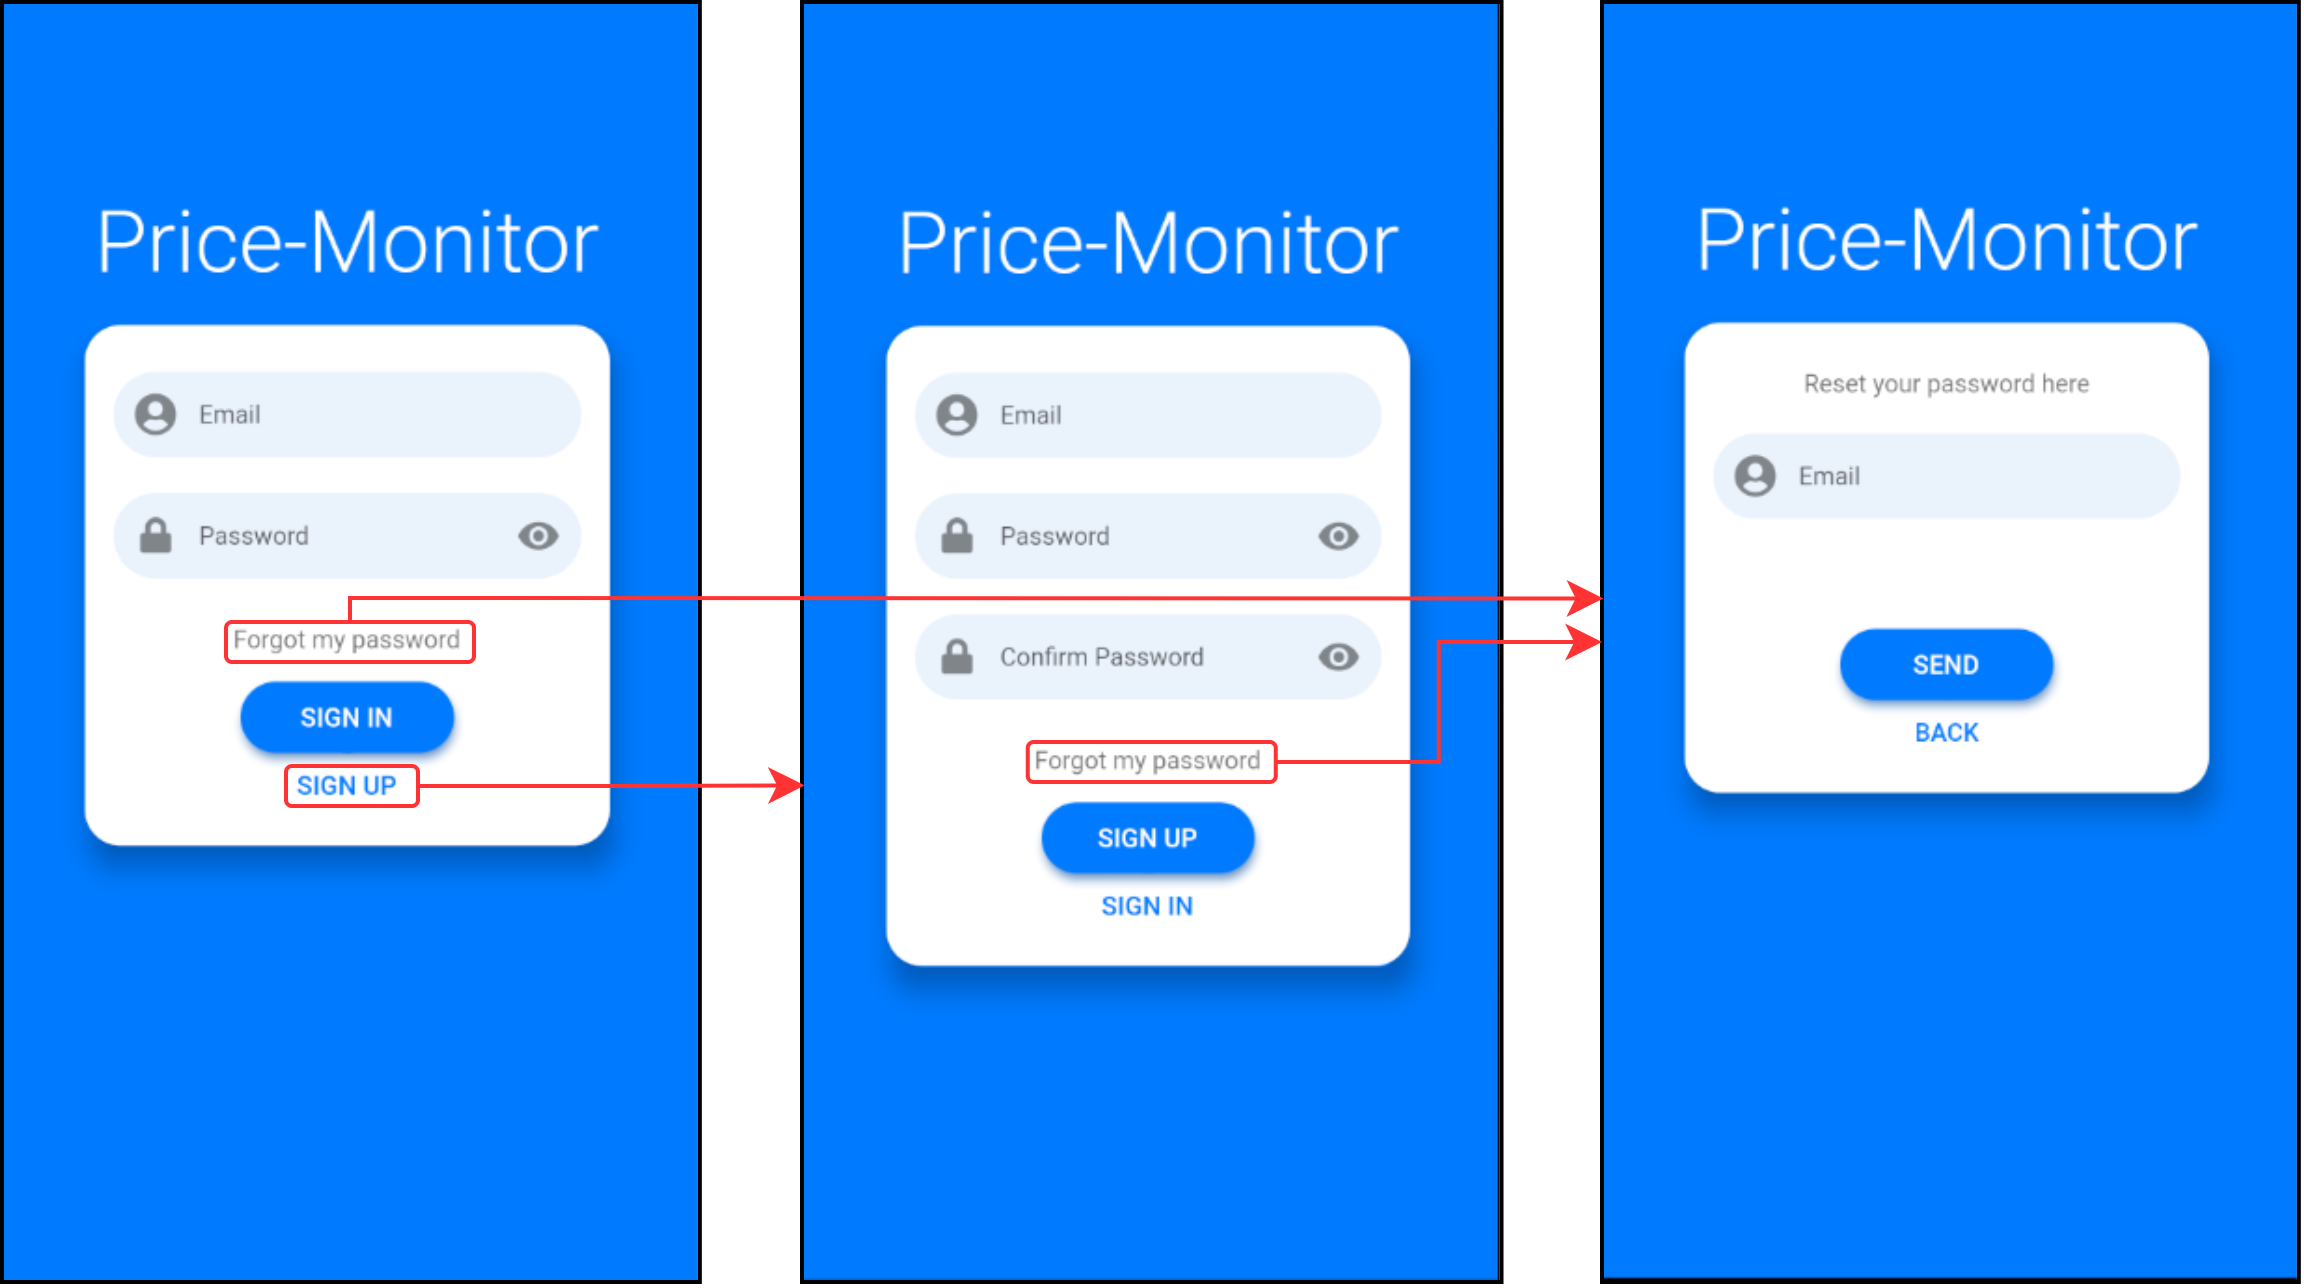
\includegraphics[scale=1]{figures/images/flutter_login.png}
    \caption{Telefonos alkalmazás bejelentkezési/regisztrálási felülete}
    \label{fig:flutter_login_reg}
\end{figure}

A bejelentkezés, regisztrálás a Firebase segítségével lett megvalósítva, melyek nagyon egyszerűvé és biztonságossá teszik ezeket a funkciókat. A jelszavak titkosítva tárolódnak az adatbázisban, ezáltal ezek ismeretlenek az adatbázist kezelő személyzetnek is. A könyvtár csomag biztosítja számunkra továbbá a jelszavak cseréjét, amennyiben elfelejtettük a régit vagy csak egyszerűen cserélni szeretnénk. Az ezeket megvalósító függvényeket és használatukat a \ref{lst:flutter_login_functions} kódrészlet illusztrálja.

\begin{lstlisting}[caption={Bejelentkező/regisztráló/jelszó csere funkciót megvalósító függvények}, label={lst:flutter_login_functions}, basicstyle=\footnotesize]
    // Sign in
    await _auth.signInWithEmailAndPassword(email: data.name, password: data.password);
    
    // Register
    await _auth.createUserWithEmailAndPassword(email: data.name, password: data.password);
    
    // Reset Password
    await _auth.sendPasswordResetEmail(email: email);
\end{lstlisting}

A felület készítésekor az egységesség játszott nagy szerepet, ezért túlnyomó részben ugyanazt a design nyelvet követtük, mint a már bemutatott böngészős kiegészítő esetében, de telefonos formára igazítva. Ennek megfelelően, a bejelentkezés után szintén egy görgethető listában láthatja a felhasználó a követett termékeit, mint azt a \ref{fig:flutter_home_info_user} ábra is mutatja. A felhasználó számara ugyanúgy rendelkezésére áll egy információs, valamint egy a felhasználói fiókjához kapcsolódó menüpont melyek a fejlécben kaptak helyet. Funkciójuk az alkalmazás rövid leírása, támogatott weboldalak listázása, valamint a felhasználó fiókjához tartozó műveletek elérése (\ref{fig:flutter_home_info_user} ábra).

\begin{figure}[H]
    \centering
    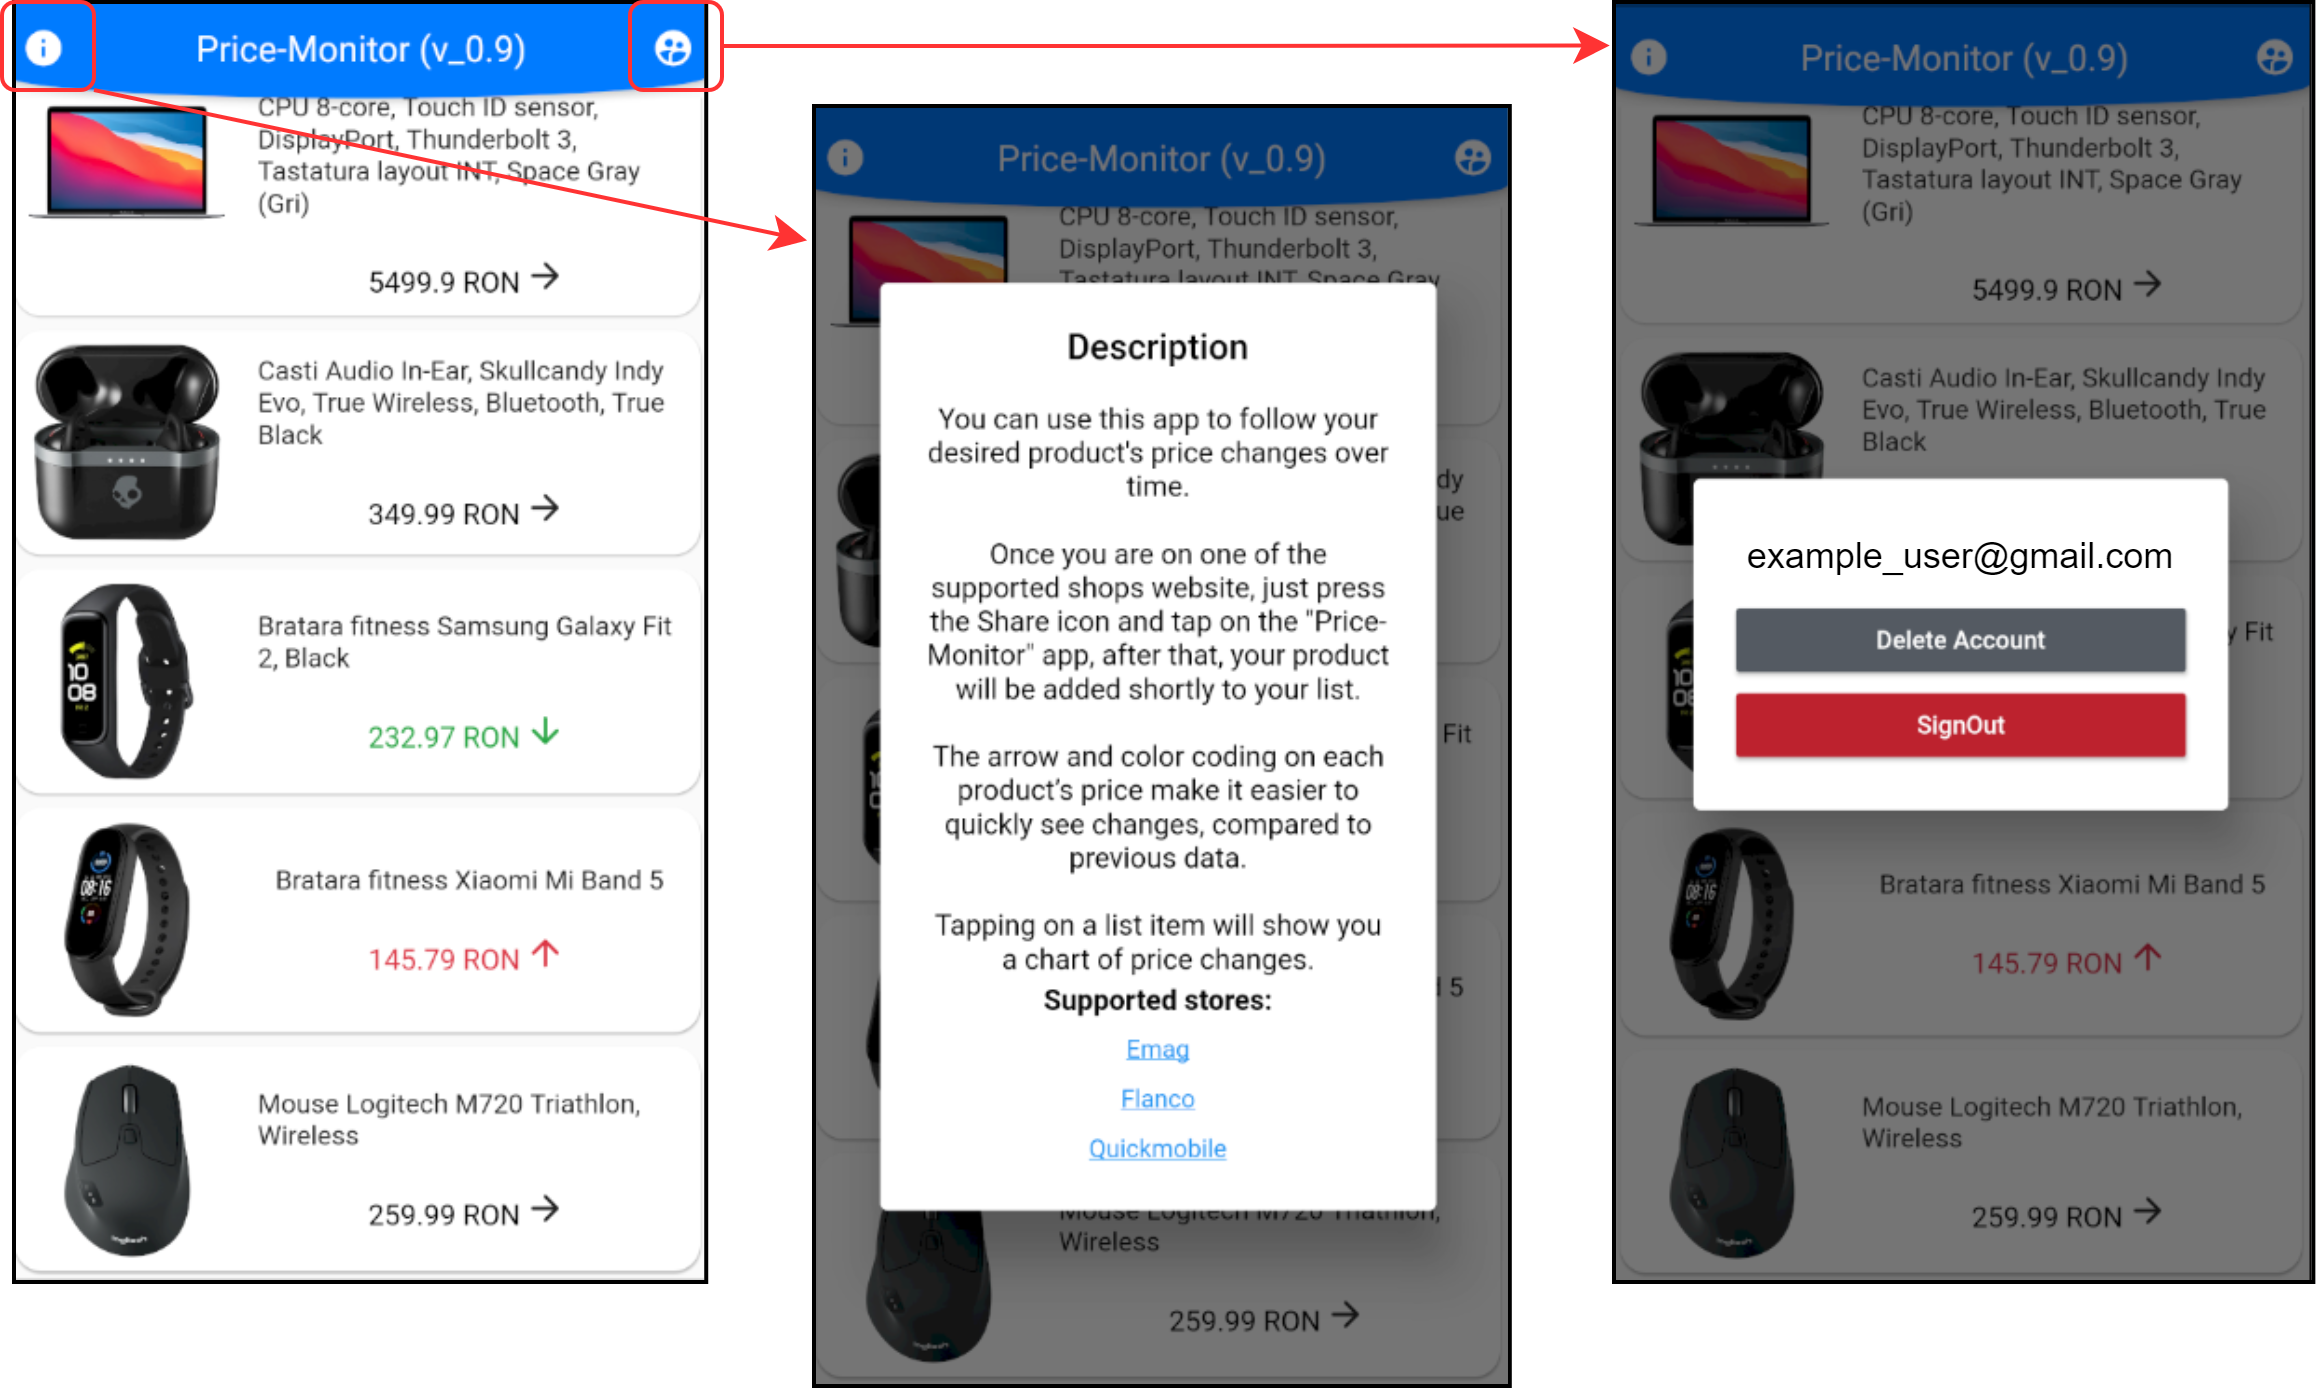
\includegraphics[scale=1]{figures/images/flutter_home_info_user.png}
    \caption{Főoldal, adminisztrációs rész}
    \label{fig:flutter_home_info_user}
\end{figure}

Egy termék hozzáadása a telefon megosztási menüjéből történik. Ehhez, az adott webshop oldalán kell lennünk, vagy amennyiben az adott oldal rendelkezik telefonos alkalmazással, mint például az Emag esetében, akkor ezt a funkciót onnan is el lehet érni. Ha megtaláltuk a követni kívánt terméket, a telefon megosztási menüjében ki kell választani az alkalmazás ikonját, ahogy ezt a \ref{fig:flutter_add} ábra mutatja. Miután ez megtörtént, át is kerülünk az alkalmazásba, ahol egy felrúgó ablakban jelenik meg számunkra, hogy biztosan hozzá szeretnénk-e adni az adott terméket. Amennyiben ezt jóváhagytuk az “Add” gomb megnyomásával, pillanatokon belül láthatjuk is a termékünket a lista alján (\ref{fig:flutter_add}).

\begin{figure}[H]
    \centering
    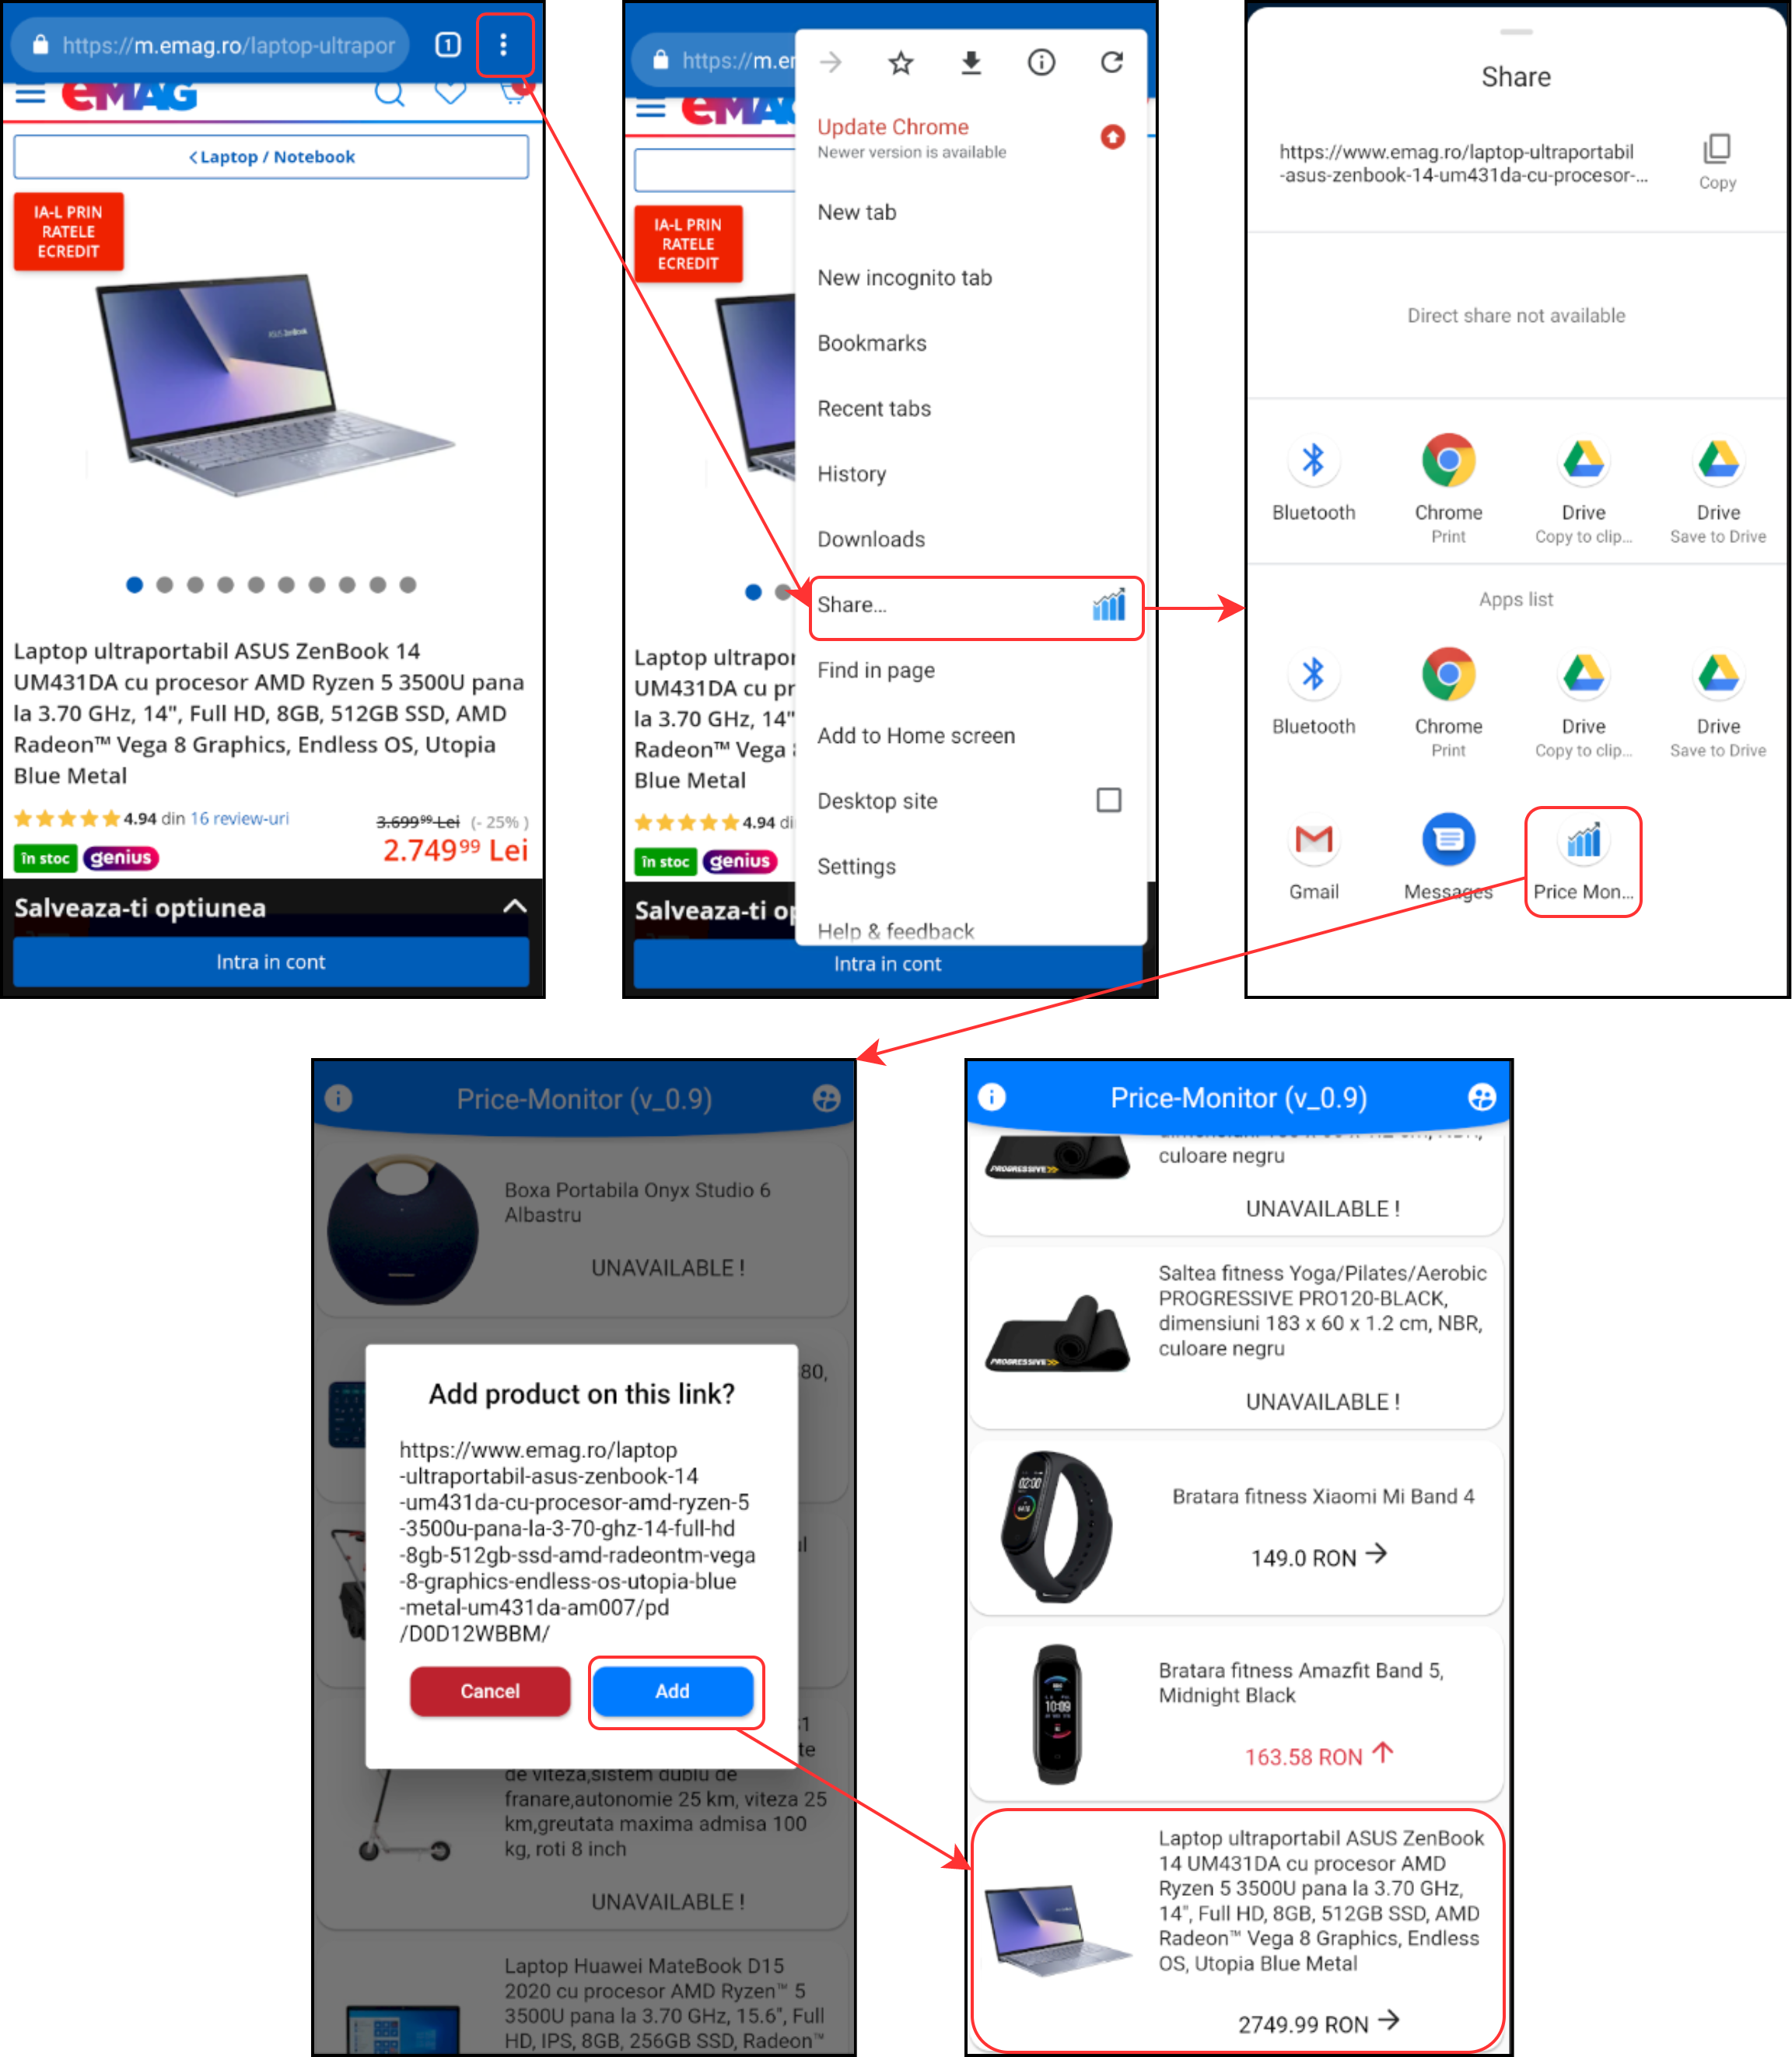
\includegraphics[scale=1]{figures/images/flutter_add.png}
    \caption{Termék hozzáadása}
    \label{fig:flutter_add}
\end{figure}

Ebben az esetben is, a termékek árainak színe, illetve a mellettük található nyíl jelképezi, hogy az ár hogyan változott az utolsó ellenőrzés óta, a zöld szín, valamint lefele irányuló nyíl csökkenést, a piros szín, felfele irányuló nyíllal drágulást, az egyenesen irányított nyíllal pedig az ár változatlanságát jelképezni. Amennyiben a termék nem elérhető, az ár helyét az „UNAVAILABLE” szöveg veszi át. Amikor egy elemet kiválasztunk a listából, az alkalmazás átvisz minket egy másik oldalra, ahol az árak változását láthatjuk egy diagram formájában. A diagram alapértelmezetten az elmúlt heti változásokat mutatja, viszont a diagram alatt található gombok segítségével változtathatjuk az idő skálát, a heti szint mellett hónapos vagy a teljes adathalmaz ábrázolása érdekében, melyek működését a \ref{fig:flutter_chart} ábrán lathatjuk.

\begin{figure}[H]
    \centering
    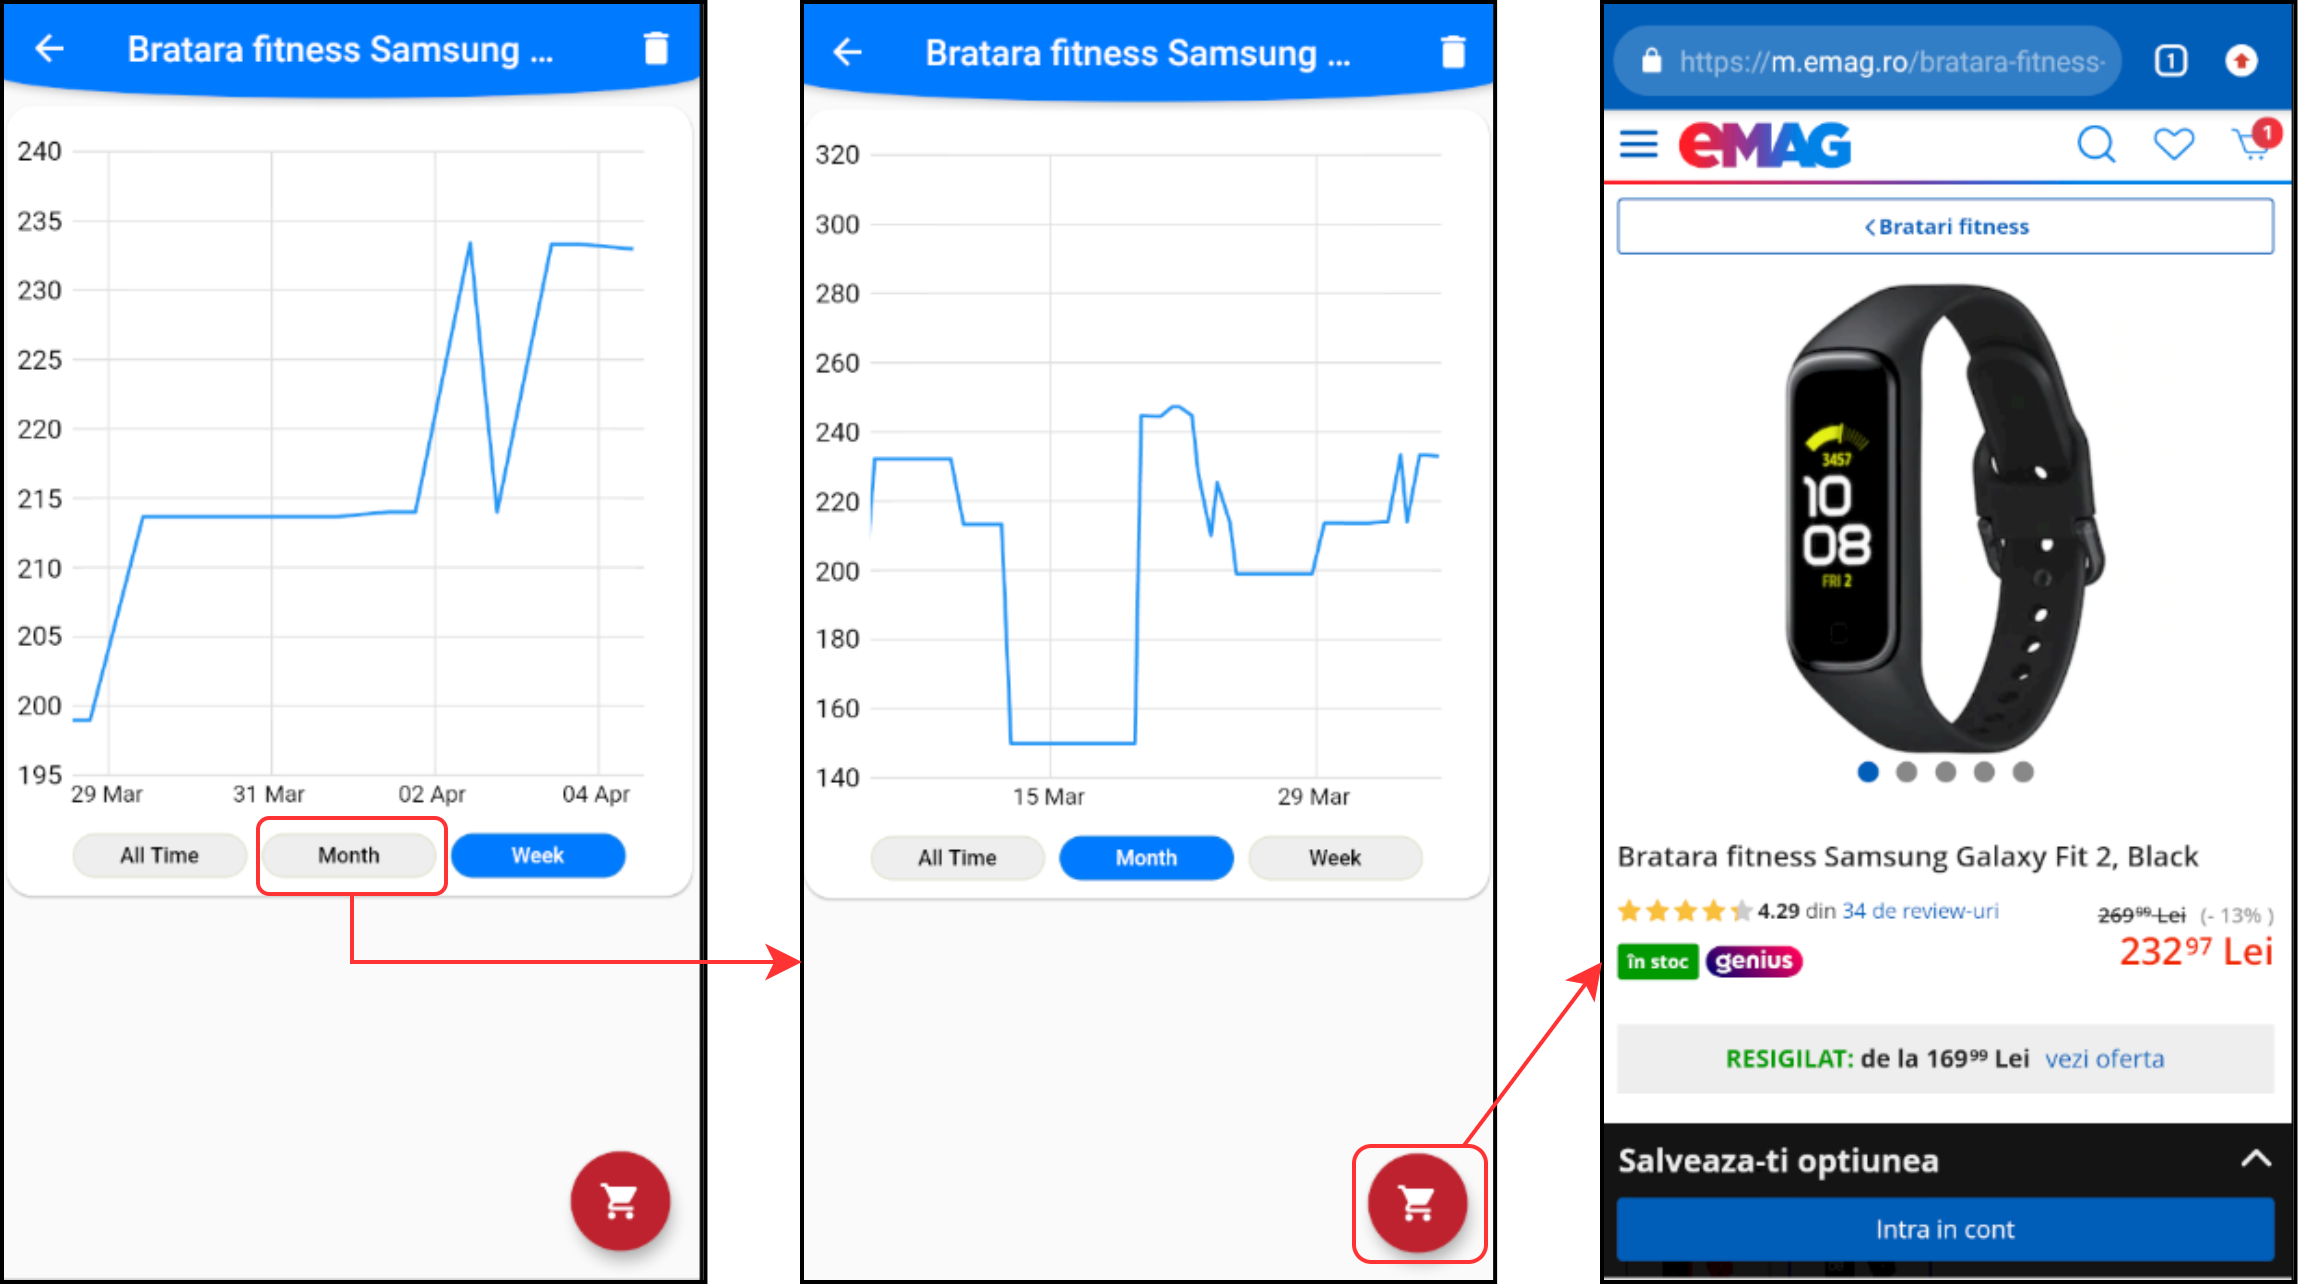
\includegraphics[scale=1]{figures/images/flutter_chart.png}
    \caption{Termék árváltozása}
    \label{fig:flutter_chart}
\end{figure}

Az ablak jobb alsó sarkában található egy bevásárló kosárral jelölt gomb, melyet, ha megnyomunk az alkalmazás átirányít minket és a telefon alapértelmezett böngészőjében megnyitja nekünk a termék weboldalát (\ref{fig:flutter_chart}). Amennyiben már nem vagyunk érdekeltek a termék követésesben, a jobb felső sarokban található, kukával jelölt gombbal törölhetjük azt a követési listánkból.

Ha egy nem támogatott oldal termekét próbáljuk meg hozzáadni, akkor egy felrúgó úgynevezett „toast” üzenetben az alkalmazás közli a felhasználóval hogy nem támogatott oldalról van szó a "Store not supported!" szöveggel, ugyanakkor ha már követi az adott terméket, akkor annak megfelelő „Product already followed!” szöveget ír ki, ezek megvalósítása és működése a \ref{lst:flutter_add_error} kódrészletben és a  \ref{fig:flutter_add_error} ábrán láthatóak.

\begin{lstlisting}[caption={Informáló üzeneteket megjelenítő függvények}, label={lst:flutter_add_error}, basicstyle=\footnotesize]
    // Ha mar kovetjuk a termeket
    Fluttertoast.showToast(msg: "Product already followed!", toastLength: Toast.LENGTH_LONG);

    // Ha nem tamogatott oldalrol szeretnenk termeket hozzaadni
    Fluttertoast.showToast(msg: "Store not supported!", toastLength: Toast.LENGTH_LONG);
\end{lstlisting}

\begin{figure}[H]
    \centering
    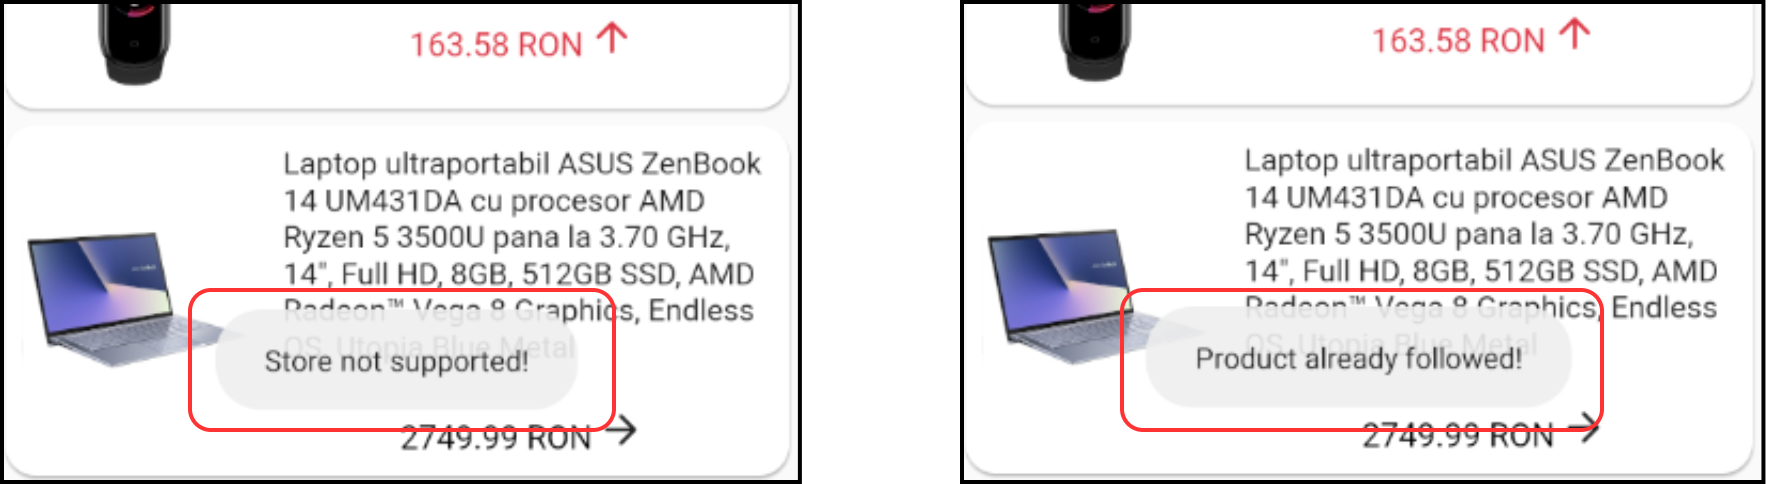
\includegraphics[scale=1]{figures/images/flutter_add_error.png}
    \caption{Informáló üzenetek}
    \label{fig:flutter_add_error}
\end{figure}

\subsection{Backend}

A rendszer backend részéért egy Python script valósítja meg. Ez Python3-as nyelven íródott, felhasználva több, a célnak megfelelő függvény könyvtárat, mint például request: a http kérések intézéséhez, BeautifulSoup: a HTML kódban való kereséshez, különböző Firebase függvény könyvtárak: az egyes adatbázissal kapcsolatos műveletek megvalósítására, Schedule: az időszakos ellenőrzések automatizálására, valamint logging: az események naplózására, valamint terminálra való egységes rendezett kiírására.

A rendszernek ez a része felelős a termékek hozzáadásáért, azok árainak frissítéséért. Ez úgy történik, hogy lekéri az adatbázisból a termékek URL-jét, majd ezekhez egy HTTP kérést intéz. Az adott weboldal visszaküldi a megjelenítéshez szükséges HTML kódot, melyet aztán a BeautifulSoup függvény könyvtár segítségével, egy elemenként kereshető formátumra alakítja. Ebben már tulajdonképpeni HTML tag-ekre kereshetünk, megadva bizonyos tulajdonságaikat, ezekből kinyerjük a számunkra szükséges információkat, amik a termék megnevezése, ára, valamint egy hozzá tartozó kép. A rendszer ezekhez társítja az ellenőrzés időpontját, majd ez feltöltésre kerül az adatbázisba, a megfelelő felhasználóhoz kötve. 

A script terminálban fut, indítás után kiválaszthatjuk milyen futási módban szeretnénk indítani (\ref{fig:python_start} ábra). Ezek a Continuous vagy folytonos, illetve az Update. A folytonos mód kiválasztása esetén a rendszer elindítja az új termékek hozzáadását figyelő és az ütemezett ellenőrzésekért felelős modulokat. Az új termékek hozzáadásáért felelős modul folyamatosan figyeli, hogy az adatbázis részéről érkezett-e valamiféle jelzés. Amennyiben egy új terméket akarunk hozzáadni az alkalmazásokon keresztül, ahogy azt az előbbi modulok tárgyalásánál láthattuk, a követni kívánt termék hozzáadásra kerül az adatbázisba, ami ezek után jelzést küld a Python scriptnek. Amint megérkezett a jelzés, azonnal elkezdődik az adatok kinyerése és hozzáadása a felhasználó listájához, az előzőekben tárgyalt módon. Az ütemezett ellenőrzésekért felelős modul segítségével, előre meghatározott időpillanatokban elindul az árak frissítése, amely az adatbázisban található összes termék árát frissíti. Ezen a modulon belül találatunk egy az internetkapcsolatot figyelő részt is, amely egy esetleges kapcsolat megszűnése esetén azonnal próbál újrakapcsolódni, amint ez sikerül, újraindítja a rendszer funkcióit, amelyek esetleg leálltak az internetkapcsolat megszűnésekor. Az Update módot kiválasztva, a rendszer azonnal elkezdi az összes termék frissítését, lásd \ref{fig:python_start} ábra, majd miután végzett, automatikusan folytatja a futást folytonos módban. Az ehhez tartozó megvalósítás a \ref{lst:python_start} kódrészleten látható.

\begin{figure}[H]
    \centering
    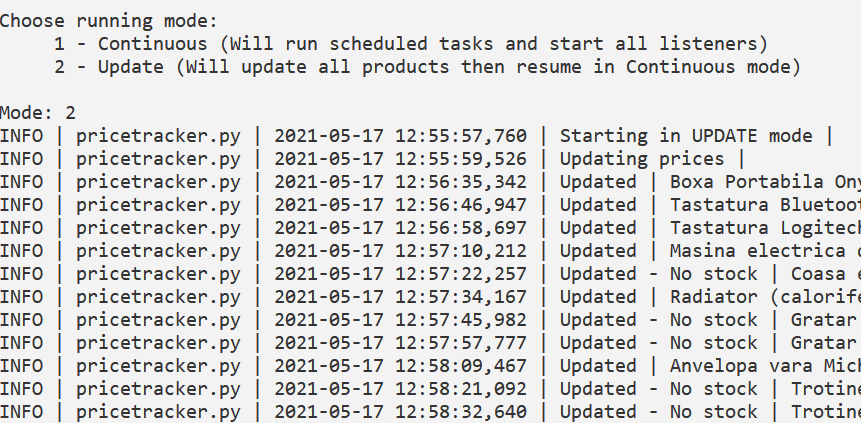
\includegraphics[scale=0.9]{figures/images/python_start.png}
    \caption{Python script Update módban való indítása}
    \label{fig:python_start}
\end{figure}

\begin{lstlisting}[caption={Backend szolgáltatás indítása}, label={lst:python_start}, basicstyle=\footnotesize]
    def run(mode):
    try:
        if mode is None:
            print("\nChoose running mode:\n"
                  "     1 - Continuous (Will run scheduled tasks and start all listeners)\n"
                  "     2 - Update (Will update all products then resume in Continuous mode)\n")
            mode = int(input("Mode: "))

        if (mode != 1) and (mode != 2):
            print("Invalid option, please select again!")
            return run(None)
        else:
            if mode == 1:
                logger.info("Starting in CONTINUOUS mode")
                run_new_products_listener()
                run_scheduled_checks()
            if mode == 2:
                logger.info("Starting in UPDATE mode")
                update_prices()
                logger.info("All products updated, starting CONTINUOUS mode!")
                run_new_products_listener()
                run_scheduled_checks()
    except Exception as error:
        logging.critical("Error while starting service!" + str(error))
        for i in range(5, 0, -1):
            logger.info("Retrying in... " + str(i) + " seconds")
            time.sleep(1)
        return run(mode)
\end{lstlisting}

Amint az előbbiekben szó volt, a BeautifulSoup nevű függvénykönyvtár segítségével lesznek kinyerve a szükséges információk, a weboldalak HTML kódjából. Ez a művelet a „find” nevű függvénnyel történik, melynek meg kell adni két paramétert. Az egyik, hogy milyen típusú tag-eket szeretnénk keresni, mint például, div, span, h1, p, a másik pedig hogy ezek milyen tulajdonságokkal rendelkeznek, például a tag egy bizonyos osztálynévvel van ellátva. A \ref{lst:python_emag} kódrészlet tartalmazza egy termék adatainak feldolgozását, amennyiben az, az Emag webáruházról származik. 

\begin{lstlisting}[caption={Emag linket feldolgozó függvény}, label={lst:python_emag}, basicstyle=\footnotesize]
    def get_and_parse_emag(soup):
    title = find_title(soup, "h1", "page-title")
    out_of_stock = soup.find("span", attrs={"class": "label-out_of_stock"})

    if out_of_stock or (title is constants.error):
        price = constants.error
    else:
        try:
            form = soup.find("form", attrs={"class": "main-product-form"})
            price = form.find("p", attrs={"class": "product-new-price"}).text.strip()
            s = list(price)
            s.insert(-6, ",")
            price = "".join(s)
            price = re.sub("Lei", '', price)
            price = re.sub("\.", "", price)
            price = re.sub(",", ".", price)
            try:
                price = float(price.strip())
            except ValueError:
                price = re.sub("de la", "", price)
                try:
                    price = float(price.strip())
                except ValueError:
                    price = constants.error
        except AttributeError:
            price = constants.error
    prod_currency = currency.ron
    try:
        image = soup.find("div", attrs={"id": "product-gallery"}).img["src"]
    except AttributeError:
        image = "error"
    product_data = class_ProductData.ProductData(title, price, prod_currency, image)
    return product_data
\end{lstlisting}

\subsection{Web áruházak}

A rendszer fontos részét képezik maguk a web áruházak is, hiszen ezek biztosítják számunkra a szükséges adatokat. A weboldalak HTML nyelven felépített elemekből állnak, melyeket a böngészőnk megjelenít számunkra. Ezt a struktúrát bárki megtekintheti, ha egy weboldalon tartózkodva megnyomja az F12 billentyűt, vagy egy jobb klikket követően az Inspect opciót kiválasztva. Amint azt korábban is említettük, az alkalmazás ezek között a struktúrák között keresi a számunkra értékes információt. Hogy ezt hogyan is találjuk meg, azt a \ref{fig:inspect_screenshot} ábrán láthatjuk is. Ezen egy termék ára lett kijelölve, majd az előbb említett Inspect opció lett kiválasztva. A böngészőnk ki is adta, hogy a kijelölt információ egy <p> tag alatt található, amely egy „product new price” osztálynévvel van ellátva. Az alkalmazás pontosan ezeket az információkat bányássza ki egy weboldal struktúrájából, legyen az az ár, a megnevezés vagy akár a társított kép elérhetősége.

\begin{figure}[H]
    \centering
    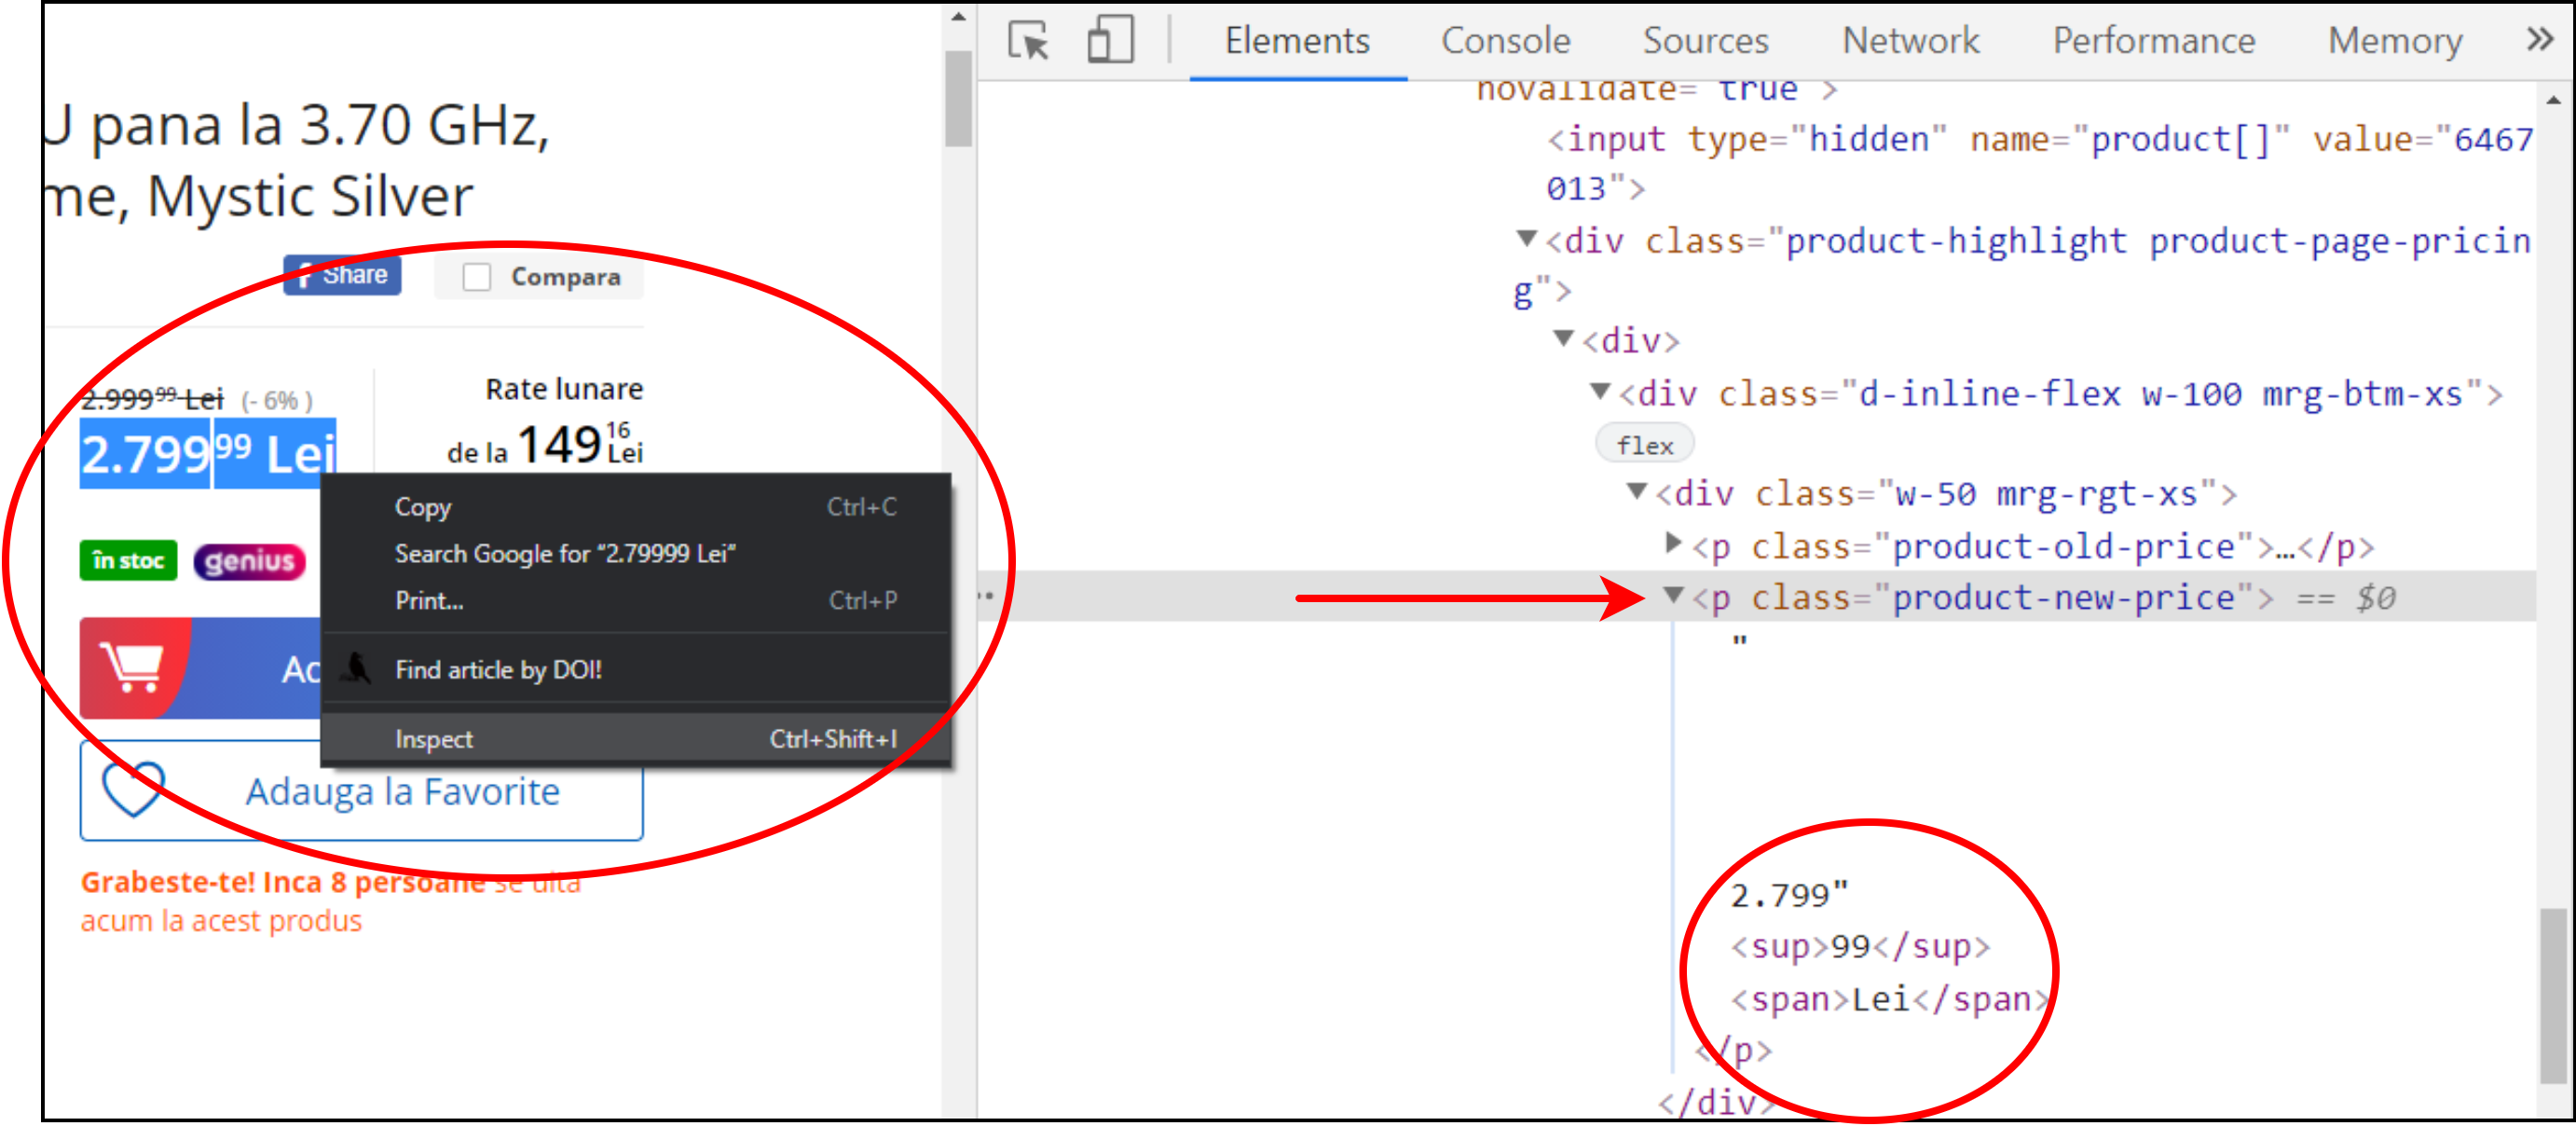
\includegraphics[scale=0.45]{figures/images/inspect_screenshot.png}
    \caption{Információ lokalizálása a weboldal strukturájában - Emag}
    \label{fig:inspect_screenshot}
\end{figure}

Mivel minden weboldal más struktúrával rendelkezik, ezért az ezeken található információ is másképp van elrendezve. Bármilyen weboldalon szeretnénk keresni, nagy valószínűséggel mindegyiknek más, egyedi struktúrája lesz (lásd \ref{fig:webshop_different_structure} ábra), ezért ezeket személyre szabottan kell kezelni. Ugyanakkor, előfordulnak változások is a struktúrában, ezért ezeket folyamatosan figyelni kell és el kell végezni a szükséges változtatásokat, annak érdekében, hogy a szoftver helyesen működjön. 

\begin{figure}[H]
    \centering
    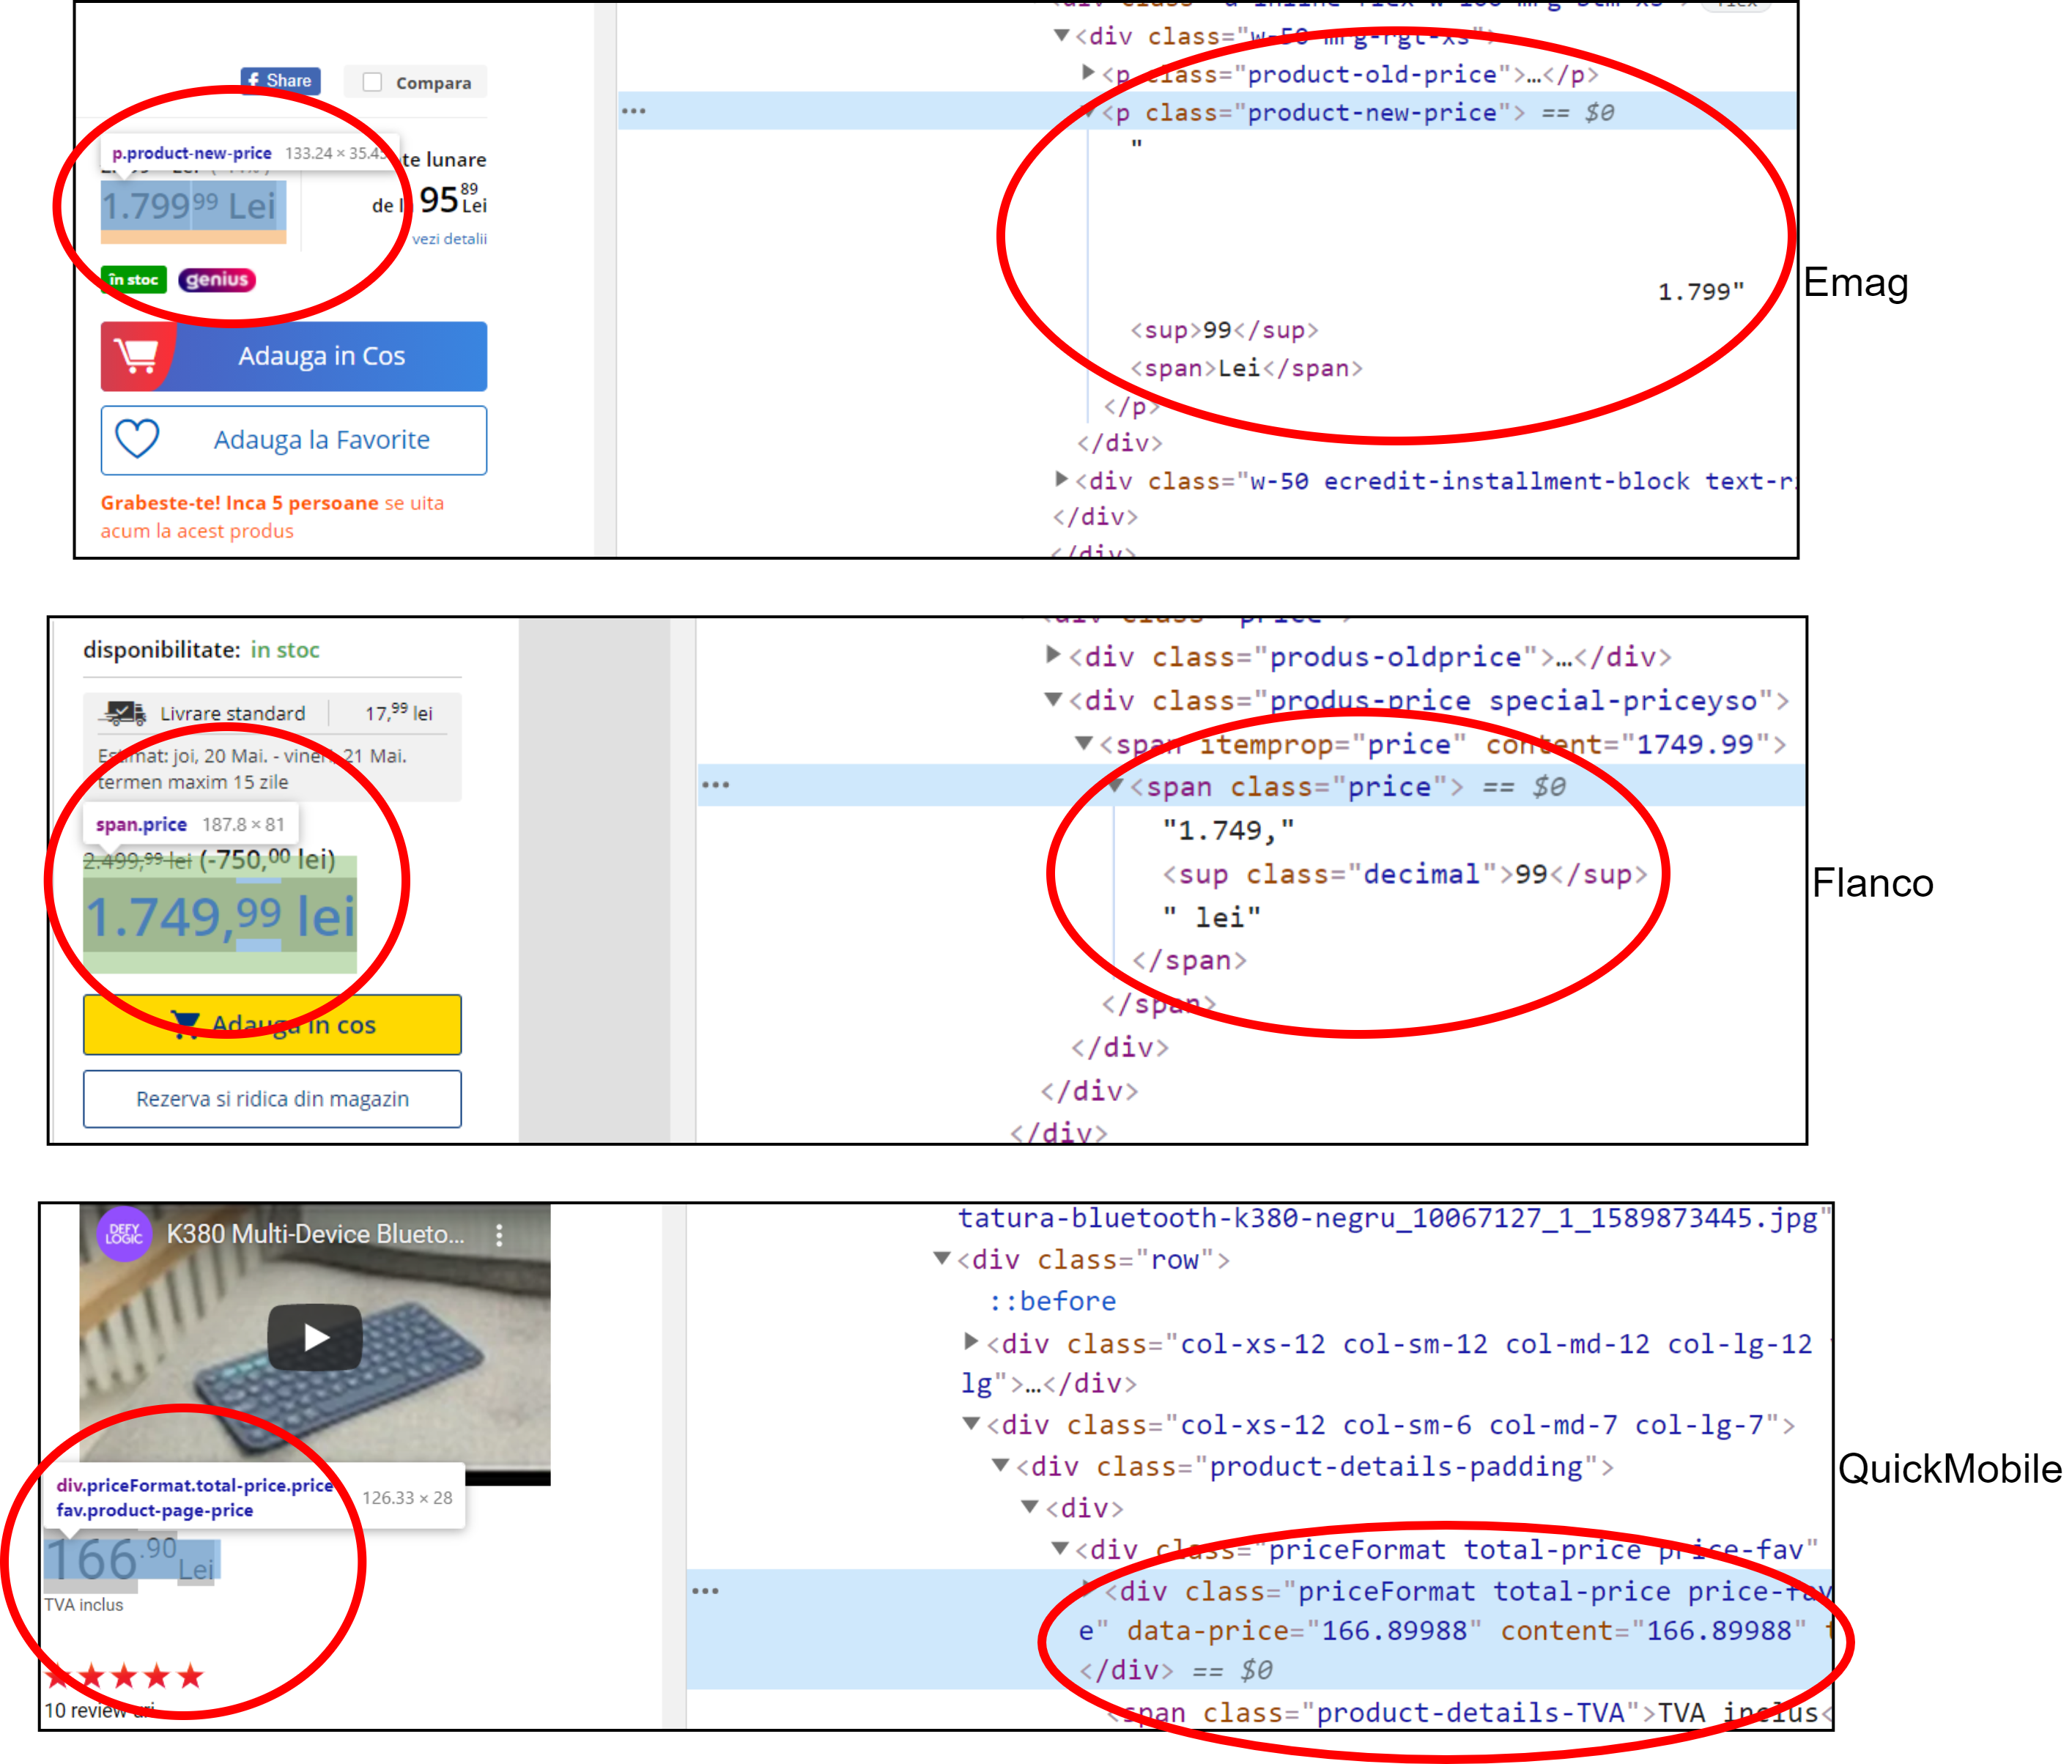
\includegraphics[scale=0.95]{figures/images/webshop_different_structure.png}
    \caption{Támogatott weboldalak különböző strukturája}
    \label{fig:webshop_different_structure}
\end{figure}

\subsection{Adatbázis}

Az rendszer adatbázisként a Firebase Realtime Database-t használja. Ez az adatbázis a Google platform által biztosított valós idejű adatbázis, amely számos funkcióval rendelkezik. Egy NoSQL adatbázisról van szó, amely az adatokat egy JSON formátumhoz hasonló struktúrában tárolja, ezáltal megkönnyítve a használatát, valamint az integrációt az egyes programozási nyelvek esetében. A rendszer valós idejűsége miatt, az adatok azonnal szinkronizálódnak az összes felhasználó között, igy mindig a legaktuálisabb adatokat látjak.